% Options for packages loaded elsewhere
\PassOptionsToPackage{unicode}{hyperref}
\PassOptionsToPackage{hyphens}{url}
\PassOptionsToPackage{dvipsnames,svgnames,x11names}{xcolor}
%
\documentclass[
  12pt,
]{article}
\usepackage{amsmath,amssymb}
\usepackage{lmodern}
\usepackage{iftex}
\ifPDFTeX
  \usepackage[T1]{fontenc}
  \usepackage[utf8]{inputenc}
  \usepackage{textcomp} % provide euro and other symbols
\else % if luatex or xetex
  \usepackage{unicode-math}
  \defaultfontfeatures{Scale=MatchLowercase}
  \defaultfontfeatures[\rmfamily]{Ligatures=TeX,Scale=1}
  \setmainfont[]{Times New Roman}
\fi
% Use upquote if available, for straight quotes in verbatim environments
\IfFileExists{upquote.sty}{\usepackage{upquote}}{}
\IfFileExists{microtype.sty}{% use microtype if available
  \usepackage[]{microtype}
  \UseMicrotypeSet[protrusion]{basicmath} % disable protrusion for tt fonts
}{}
\makeatletter
\@ifundefined{KOMAClassName}{% if non-KOMA class
  \IfFileExists{parskip.sty}{%
    \usepackage{parskip}
  }{% else
    \setlength{\parindent}{0pt}
    \setlength{\parskip}{6pt plus 2pt minus 1pt}}
}{% if KOMA class
  \KOMAoptions{parskip=half}}
\makeatother
\usepackage{xcolor}
\usepackage[margin=1in]{geometry}
\usepackage{graphicx}
\makeatletter
\def\maxwidth{\ifdim\Gin@nat@width>\linewidth\linewidth\else\Gin@nat@width\fi}
\def\maxheight{\ifdim\Gin@nat@height>\textheight\textheight\else\Gin@nat@height\fi}
\makeatother
% Scale images if necessary, so that they will not overflow the page
% margins by default, and it is still possible to overwrite the defaults
% using explicit options in \includegraphics[width, height, ...]{}
\setkeys{Gin}{width=\maxwidth,height=\maxheight,keepaspectratio}
% Set default figure placement to htbp
\makeatletter
\def\fps@figure{htbp}
\makeatother
\setlength{\emergencystretch}{3em} % prevent overfull lines
\providecommand{\tightlist}{%
  \setlength{\itemsep}{0pt}\setlength{\parskip}{0pt}}
\setcounter{secnumdepth}{-\maxdimen} % remove section numbering
\newlength{\cslhangindent}
\setlength{\cslhangindent}{1.5em}
\newlength{\csllabelwidth}
\setlength{\csllabelwidth}{3em}
\newlength{\cslentryspacingunit} % times entry-spacing
\setlength{\cslentryspacingunit}{\parskip}
\newenvironment{CSLReferences}[2] % #1 hanging-ident, #2 entry spacing
 {% don't indent paragraphs
  \setlength{\parindent}{0pt}
  % turn on hanging indent if param 1 is 1
  \ifodd #1
  \let\oldpar\par
  \def\par{\hangindent=\cslhangindent\oldpar}
  \fi
  % set entry spacing
  \setlength{\parskip}{#2\cslentryspacingunit}
 }%
 {}
\usepackage{calc}
\newcommand{\CSLBlock}[1]{#1\hfill\break}
\newcommand{\CSLLeftMargin}[1]{\parbox[t]{\csllabelwidth}{#1}}
\newcommand{\CSLRightInline}[1]{\parbox[t]{\linewidth - \csllabelwidth}{#1}\break}
\newcommand{\CSLIndent}[1]{\hspace{\cslhangindent}#1}
\usepackage{setspace}\doublespacing
\usepackage[left]{lineno}
\ifLuaTeX
  \usepackage{selnolig}  % disable illegal ligatures
\fi
\IfFileExists{bookmark.sty}{\usepackage{bookmark}}{\usepackage{hyperref}}
\IfFileExists{xurl.sty}{\usepackage{xurl}}{} % add URL line breaks if available
\urlstyle{same} % disable monospaced font for URLs
\hypersetup{
  colorlinks=true,
  linkcolor={RoyalBlue},
  filecolor={Maroon},
  citecolor={Blue},
  urlcolor={RoyalBlue},
  pdfcreator={LaTeX via pandoc}}

\author{}
\date{\vspace{-2.5em}}

\begin{document}

\pagenumbering{arabic}

Running head: Burn severity and ecosystem transformation

Title: Fuel connectivity, burn severity, and seedbank survivorship drive
ecosystem transformation in a semi-arid shrubland.

Adam L. Mahood\textsuperscript{1,2,3,\texttt{*}}, Michael J.
Koontz\textsuperscript{2}, Jennifer K. Balch\textsuperscript{1,2,4}

\small

\textsuperscript{1} Department of Geography, University of Colorado
Boulder, Boulder, CO, USA

\textsuperscript{2} Earth Lab, University of Colorado, Boulder, CO, USA

\textsuperscript{3} Water Resources, Agricultural Research Service,
United States Department of Agriculture, Fort Collins, CO, USA

\textsuperscript{4} Environmental Data Science Innovation and Inclusion
Lab, University of Colorado, Boulder, CO

\texttt{*} Corresponding author:
\href{mailto:admahood@gmail.com}{\nolinkurl{admahood@gmail.com}}

\normalsize

Open Research Statement: Data and code to recreate the analysis are
freely available at \url{https://doi.org/10.5281/zenodo.5293996}.

\newpage

\linenumbers

\hypertarget{abstract}{%
\subsection{Abstract}\label{abstract}}

A key challenge in ecology is understanding how multiple drivers
interact to precipitate persistent vegetation state changes. These state
changes may be both precipitated and maintained by disturbances, but
predicting whether the state change is fleeting or persistent requires
an understanding of the mechanisms by which disturbance affects the
alternative communities. In the sagebrush shrublands of the western
United States, widespread annual grass invasion has increased fuel
connectivity, which increases the size and spatial contiguity of fires,
leading to post-fire monocultures of introduced annual grasses (IAG).
The novel grassland state can be persistent, and more likely to promote
large fires than the shrubland it replaced. But the mechanisms by which
pre-fire invasion and fire occurrence are linked to higher post-fire
flammability are not fully understood. A natural experiment to explore
these interactions presented itself when we arrived in northern Nevada
immediately after a 50,000 ha wildfire was extinguished.

We hypothesized that the novel grassland state is maintained via a
reinforcing feedback where higher fuel connectivity increases burn
severity, which subsequently increases post-fire IAG dispersal, seed
survivorship, and fuel connectivity. We used a Bayesian joint species
distribution model and structural equation model framework to assess the
strength of the support for each element in this feedback pathway. We
found that pre-fire fuel connectivity increased burn severity and that
higher burn severity had mostly positive effects on the occurrence of
IAG and another non-native species, and mostly negative or neutral
relationships with all other species. Finally, we found that the
abundance of IAG seeds in the seedbank immediately post-fire had a
positive effect on the fuel connectivity 3 years after fire, completing
a positive feedback promoting IAG. These results demonstrate that the
strength of the positive feedback is controlled by measurable
characteristics of ecosystem structure, composition and disturbance.
Further, each node in the loop is affected independently by multiple
global change drivers. It is possible that these characteristics can be
modeled to predict threshold behavior and inform management actions to
mitigate or slow the establishment of the grass-fire cycle, perhaps via
targeted restoration applications or pre-fire fuel treatments.

\emph{Keywords}: \emph{Artemisia tridentata}, alternative stable states,
\emph{Bromus tectorum}, burn severity, cheatgrass, fuel connectivity,
grass-fire cycle, joint species distribution model, resilience,
sagebrush

\hypertarget{introduction}{%
\subsection{1. Introduction}\label{introduction}}

Ecosystems around the world are being affected simultaneously by
multiple facets of global change. For example, changes in land use can
facilitate exotic plant invasions
(\protect\hyperlink{ref-Allan2015}{Allan et al. 2015}), which can alter
ecosystem structure (\protect\hyperlink{ref-Davies2013}{Davies and Nafus
2013}). Altered structure can change the likelihood of a disturbance,
the properties of a disturbance and the capacity of the system to
recover after a disturbance (\protect\hyperlink{ref-Brooks2004}{Brooks
et al. 2004}). Global climate change can also directly affect the
magnitude of disturbances (\protect\hyperlink{ref-Parks2020}{S. A. Parks
and Abatzoglou 2020}), and act as a demographic filter that influences
how ecosystems recover after disturbances
(\protect\hyperlink{ref-Rother2015}{Rother, Veblen, and Furman 2015};
\protect\hyperlink{ref-Davis2019}{Davis et al. 2019}) via impacts on
adult plant survival and seed dispersal
(\protect\hyperlink{ref-Davis2018}{Davis, Higuera, and Sala 2018};
\protect\hyperlink{ref-Eskelinen2020}{Eskelinen et al. 2020}). The
combined effects of global change forces on structure, function and
disturbance can cascade and interact. For example, while burn severity
(or the proportion of biomass burned
(\protect\hyperlink{ref-Keeley2009}{Keeley 2009})) is influenced by
vegetation structure (\protect\hyperlink{ref-Koontz2020}{Koontz et al.
2020}; \protect\hyperlink{ref-Parks2018}{Sean A. Parks et al. 2018}), it
also increases with temperature and aridity
(\protect\hyperlink{ref-Parks2020}{S. A. Parks and Abatzoglou 2020}).
These forces can ultimately lead to permanent compositional change,
biodiversity losses and the loss of ecosystem services
(\protect\hyperlink{ref-Ratajczak2018}{Ratajczak et al. 2018};
\protect\hyperlink{ref-Mahood2019}{Mahood and Balch 2019};
\protect\hyperlink{ref-Mahood2021}{Mahood et al. 2022}) due to internal,
self-reinforcing mechanisms that arise from those structural and
functional changes which then maintain an alternative stable state
(\protect\hyperlink{ref-Scheffer2003}{Marten Scheffer and Carpenter
2003}; \protect\hyperlink{ref-Ratajczak2018}{Ratajczak et al. 2018}).

There is a long history of univariate time series observations that show
sudden state changes (\protect\hyperlink{ref-Scheffer2003}{Marten
Scheffer and Carpenter 2003}), and these have informed the development
of theories that help us understand how systems of any type can change
state suddenly, and exist in persistent alternative stable states
(\protect\hyperlink{ref-Scheffer2015}{Marten Scheffer et al. 2015};
\protect\hyperlink{ref-Ratajczak2018}{Ratajczak et al. 2018}). These
theories typically represent the system's state with a single variable,
of which the mean is observed to abruptly change in time or space
(\protect\hyperlink{ref-Scheffer2015}{Marten Scheffer et al. 2015}).
Descriptive evidence of alternative stable states has been documented at
broad scales in tropical ecosystems, where forests, savannas and
grasslands are considered alternative stable states because they are
floristically distinct (\protect\hyperlink{ref-Aleman2020}{Aleman et al.
2020}) and cluster around static values of woody cover (80, 30 and 0
percent) while occurring along overlapping ranges of precipitation
(\protect\hyperlink{ref-Hirota2011}{Hirota et al. 2011};
\protect\hyperlink{ref-Staver2011}{Staver, Archibald, and Levin 2011}).
The forested state has a self-reinforcing, positive feedback between
evapotranspiration and tree cover
(\protect\hyperlink{ref-Staal2020}{Staal et al. 2020}), while the
grassland and savanna states are maintained by feedbacks between grass
flammability and fire occurrence
(\protect\hyperlink{ref-DAntonio1992}{D'Antonio and Vitousek 1992};
\protect\hyperlink{ref-Staver2011}{Staver, Archibald, and Levin 2011}).
Alternative stable states are believed to be widespread
(\protect\hyperlink{ref-Scheffer2001}{M. Scheffer et al. 2001}), but
their existence is rarely proven at broader scales, with most
demonstrative studies having been conducted in greenhouse and laboratory
microcosm experiments (\protect\hyperlink{ref-Schroder2005}{Schröder,
Persson, and De Roos 2005}). One of the reasons for this is that
ecological systems are much more complex than a simple bivariate system
with a single driver and a single response. There may be multiple
drivers, and the state is the product of interactions between organisms
and their immediate environment, as well as countless inter- and
intra-specific interactions.

A central challenge in ecology in the 21st century is to move from
describing how plant communities are affected by global change to the
capacity to predict how species pools will assemble and persist in
response to global change (\protect\hyperlink{ref-Davis2018}{Davis,
Higuera, and Sala 2018}; \protect\hyperlink{ref-Keddy2021}{Keddy and
Laughlin 2021}). Prediction of community response to multi-faceted
global change drivers is enhanced with a better understanding of the
mechanisms that underlie community stability in the face of
disturbances. A classic example of an ecosystem that appears to have
disturbance-mediated alternative stable states (but see Morris and Leger
(\protect\hyperlink{ref-Morris2016}{2016})), but whose stability
mechanisms aren't well understood is the invasion of \emph{Bromus
tectorum} L. and other introduced annual grasses in the Great Basin of
the western United States. Here, it is well documented how the
interaction of annual grass invasion, fire
(\protect\hyperlink{ref-Balch2013}{Balch et al. 2013}) and grazing
(\protect\hyperlink{ref-Williamson2019}{Williamson et al. 2019}) are
associated with the degradation or loss of over half of Wyoming big
sagebrush (\emph{Artemisia tridentata} ssp. \emph{wyomingensis} Beetle
\& Young) ecosystems (\protect\hyperlink{ref-Davies2011}{Davies et al.
2011}). These systems had a precolonial fire regime of infrequent,
patchy fires (\protect\hyperlink{ref-Bukowski2013}{Bukowski and Baker
2013}). In uninvaded areas, the space between shrubs is typically
composed of bare ground covered in biological soil crust and caespitose
perennial plants (Figure 1). Because fire does not spread readily below
a threshold of approximately 60\% cover of flammable vegetation
(\protect\hyperlink{ref-Archibald2012}{Archibald, Staver, and Levin
2012}), the low fuel connectivity in these areas limits fire spread.
Annual grass invasion increases fuel connectivity while decreasing fuel
moisture (\protect\hyperlink{ref-Brooks2004}{Brooks et al. 2004};
\protect\hyperlink{ref-Davies2013}{Davies and Nafus 2013}), leading to
increased fire size and frequency
(\protect\hyperlink{ref-Balch2013}{Balch et al. 2013}). Sagebrush stands
with high native perennial cover might need only a small amount of
additional annual grass cover to alter ecosystem structure enough to
alter the fire regime (Figure 2). After fire, the landscape is typically
dominated by introduced annual grasses. But in order to understand how
fire drives the persistence of the grassland state, we need to
understand the demographic mechanisms by which fire impacts propagule
dispersal and benefits the alternative state
(\protect\hyperlink{ref-Davis2018}{Davis, Higuera, and Sala 2018}). As
with forested systems, propagule dispersal is a key filter through which
species must pass in order to establish and persist in a post-fire
landscape (\protect\hyperlink{ref-Gill2022}{Gill et al. 2022}).

Petraitis and Latham (\protect\hyperlink{ref-Petraitis1999}{1999})
posited that the maintenance of alternate species assemblages requires
first a disturbance that removes the species from the initial assemblage
and second the arrival of the species of the alternate assemblage. One
understudied mechanism that may explain both for the
\emph{Artemisia}/\emph{Bromus} system is the interaction between the
species composition of the soil seed bank and burn severity. Because the
invading species are annual, and many of the key native plant species
are seed obligates, the seed is the key life history stage that fire
must act upon to benefit the invading plants. Seeds and seedlings are
particularly vulnerable to climate, competition and disturbance
(\protect\hyperlink{ref-Enright2015}{Enright et al. 2015}). Warmer and
drier conditions simultaneously reduce recruitment, growth, and survival
of seeds and seedlings (\protect\hyperlink{ref-Enright2015}{Enright et
al. 2015}; \protect\hyperlink{ref-Schlaepfer2014}{Schlaepfer, Lauenroth,
and Bradford 2014}), while also increasing burn severity
(\protect\hyperlink{ref-Parks2020}{S. A. Parks and Abatzoglou 2020}). In
fire prone ecosystems, seed obligate species typically have life history
strategies to cope with fires that burn at different severities
(\protect\hyperlink{ref-Maia2012}{Maia et al. 2012};
\protect\hyperlink{ref-Wright2016}{Wright, Latz, and Zuur 2016};
\protect\hyperlink{ref-Palmer2018}{Palmer, Denham, and Ooi 2018}). Soil
heating from fire affects the response of vegetation to fire
(\protect\hyperlink{ref-Gagnon2015}{Gagnon et al. 2015}), including the
capacity of seeds to remain viable after fire
(\protect\hyperlink{ref-Humphrey2001}{Humphrey and Schupp 2001}). High
severity fire can affect species that use the seedbank positively
(\protect\hyperlink{ref-Kimura2011}{Kimura and Tsuyuzaki 2011}),
negatively (\protect\hyperlink{ref-Heydari2017}{Heydari et al. 2017}),
or have no effect (\protect\hyperlink{ref-Lipoma2018}{Lipoma, Funes, and
Díaz 2018}), depending on species-specific adaptations. Both the depth
of the burn and fire temperature can affect subsequent recovery by seed
germination (\protect\hyperlink{ref-Morgan1988}{Morgan and
Neuenschwander 1988}; \protect\hyperlink{ref-Schimmel1996}{Schimmel and
Granström 1996}), as well as seed mortality and physical seed dormancy
mechanisms (\protect\hyperlink{ref-Liyanage2017}{Liyanage and Ooi
2017}).

In addition to size and frequency, exotic plant invasions can alter fire
temperature (\protect\hyperlink{ref-Brooks2004}{Brooks et al. 2004};
\protect\hyperlink{ref-Jones2015}{R. O. Jones et al. 2015}) and burn
severity. While in many cases fires that burn at higher temperatures
will also consume more biomass (i.e.~burn at higher severity), grass
fires may not always have such a relationship. Direct measurements have
shown that \emph{B. tectorum} burns at low temperatures
(\protect\hyperlink{ref-Beckstead2011}{Beckstead et al. 2011};
\protect\hyperlink{ref-Germino2016}{Germino, Chambers, and Brown 2016}),
but because it also increases horizontal fuel connectivity
(\protect\hyperlink{ref-Davies2013}{Davies and Nafus 2013}), it leads to
more contiguously burned areas and therefore higher burn severity,
despite lower fire temperatures. To benefit from fire, \emph{B.
tectorum} would need to gain a fitness benefit relative to other species

One way to achieve this is to disperse more viable seeds into the
post-fire landscape than the other species and become well-represented
in the post-fire plant assemblage (\protect\hyperlink{ref-Bond1995}{Bond
and Midgley 1995}). If the fire is patchy, this can happen through
post-fire seed dispersal (\protect\hyperlink{ref-Monty2013}{Monty,
Brown, and Johnston 2013}). Without unburned patches, seeds must survive
the fire. If the increase in fuel connectivity caused by \emph{B.
tectorum} increases the severity of fire, one way burn severity might
then influence the community composition of the post-fire seed bank to
facilitate the post-fire dominance of \emph{B. tectorum} would be to
burn a contiguous area at a temperature high enough to kill
fire-intolerant native seeds, but low enough that \emph{B. tectorum}
seeds survive and germinate more readily from fire-induced germination
cues (\protect\hyperlink{ref-Naghipour2016}{Naghipour et al. 2016};
\protect\hyperlink{ref-Fenesi2016}{Fenesi et al. 2016}). In other words,
an area with high burn severity should have a lower relative occurrence
of viable seeds of native species, and a higher relative occurrence of
the seeds of fire-tolerant introduced annual plants. This would allow
for the for the often-observed dominance of introduced annual grasses
after a few years and would result in higher fuel connectivity, closing
the positive feedback loop. Plants that are not adapted to frequent fire
would be less likely to produce seeds that are adapted to surviving
fire, or dispersal mechanisms to take advantage of the resources
available immediately after fire
(\protect\hyperlink{ref-Keeley2011}{Keeley et al. 2011}). To our
knowledge, despite several studies on the relationship between fire
occurrence and the seed bank in this system
(\protect\hyperlink{ref-Hassan1986}{Hassan and West 1986};
\protect\hyperlink{ref-Humphrey2001}{Humphrey and Schupp 2001};
\protect\hyperlink{ref-Boudell2002}{Boudell, Link, and Johansen 2002}),
no studies to date have examined the effect of burn severity on the seed
bank. Burn severity is more ecologically meaningful than fire
occurrence, and is more useful for understanding threshold effects and
stable states than a binary variable.

Here, we collected soil cores from 14 locations along the perimeter of a
large fire (the Hot Pot fire, \textasciitilde50,000 ha) immediately
after it was extinguished, in northern Nevada in July 2016. Each
location had paired burned and unburned samples. Because it burned a
large area in only three days, we could sample a broad area while being
reasonably certain that the weather conditions during the fire were
similar at all sites. Because we collected our samples immediately after
the fire was extinguished, we felt confident that the seed bank samples
did not contain seeds deposited by post-fire dispersal. We put the
samples in cold storage and germinated the seeds from those cores in a
greenhouse the following spring. In spring 2017 and fall 2019 we
collected information on vegetation structure and diversity at each
location. We tested three hypotheses in this study that are depicted in
Figure 3: (H1) Pre-fire fuel connectivity would be positively related to
burn severity; (H2) burn severity would increase the occurrence
probability of introduced annual species in the seed bank and reduce the
occurrence probability of native species; and (H3) the abundance of
post-fire \emph{B. tectorum} seeds in the seedbank would be positively
related to post-fire fuel connectivity. We examined two alternatives to
H2: (H2a), increased fuel connectivity brought on by the invasion of
annual grasses may have already depleted the diversity of the soil seed
bank before the fire occurred; and (H2b) prefire fuel connectivity is
solely reflective of annual grass cover, which drives post-fire annual
grass seed abundance. In addition, because in our study system post-fire
sites are floristically distinct from the pre-fire state
(\protect\hyperlink{ref-Mahood2019}{Mahood and Balch 2019}), typically
with near monocultures of \emph{B. tectorum}, we hypothesized that (H4)
high post-fire fuel connectivity of those near-monocultures would result
in lower aboveground species diversity due to competitive exclusion of
native plants.

\hypertarget{methods}{%
\subsection{2. Methods}\label{methods}}

\emph{2.1 Study Area}

The study was conducted in north-central Nevada the day after a large
fire (the Hot Pot Fire) was extinguished (Appendix S1, Fig. S1). The Hot
Pot Fire burned just over 50,000 hectares in less than a week. The
pre-fire landcover was predominantly \emph{B. tectorum} and Wyoming big
sagebrush plant communities. The fire occurred after the early season
plants, including \emph{B. tectorum} and \emph{Poa secunda} J. Presl,
the most abundant native understory species, had gone to seed, and
before the late season species, including Wyoming big sagebrush, had
produced flowers. Thus we were able to isolate the effect of the fire
without any confounding effects of post-fire seed dispersal, while
achieving a broad spatial extent. The sites we sampled ranged from 1,397
to 1,607 meters in elevation.

\emph{2.2 Seed Bank Sampling}

In early July 2016, we collected samples of the soil seed bank at
fourteen locations the day after the Hot Pot fire was contained. Each
site was located at the perimeter of the fire where it was clearly
delineated by a bulldozer line or in one case a narrow dirt road. We
were confident paired sites were of the same pre-fire composition
because we had been working in these areas all summer collecting data
for another study. Eleven sites were mature sagebrush communities with
no history of fire since at least 1984. Three sites had previously
burned in 1984 according to the Monitoring Trends in Burn Severity
(MTBS) fire history (\protect\hyperlink{ref-Eidenshink2007}{Eidenshink
et al. 2007}) and had high cover of \emph{B. tectorum}, but still had
scattered sagebrush cover. We used a metal stake to mark paired burned
and unburned sampling locations on each side of the perimeter, 10 m from
the nearest evidence of anthropogenic disturbance (i.e.~bulldozer
effects, footprints) associated with active fire suppression along the
perimeter. Within 3 m of each marker, we extracted twelve, 6 cm deep, 5
cm diameter, soil cores. Seeds of sagebrush generally do not fall far
(\textless30 m) from their parent plants in this system
(\protect\hyperlink{ref-Shinneman2016}{Shinneman and McIlroy 2016}), and
so they are not uniformly distributed
(\protect\hyperlink{ref-Boudell2002}{Boudell, Link, and Johansen 2002}).
In addition, seeds from \emph{B. tectorum} and \emph{Artemisia} have
different germination rates based on the micro-site they find themselves
in (i.e.~under a shrub or in the bare ground between shrubs,
\protect\hyperlink{ref-Eckert1986}{Eckert et al. 1986}). To account for
these potentially confounding effects, we placed half of the core
locations under shrubs, half in shrub interspaces, and aggregated the
cores for each site. In the burned areas, it was obvious where shrubs
had been located. Even when they were completely incinerated, their
imprint remained on the soil surface
(\protect\hyperlink{ref-Bechtold2007}{Bechtold and Inouye 2007}). To
examine the effect of seed depth, we divided each soil core into 0-2 cm
and 2-6 cm depths. Litter was aggregated with the 0-2 cm samples.
Samples were then placed in cold storage (\textasciitilde2 deg C) for 3
months (\protect\hyperlink{ref-Meyer2013}{Meyer, Monsen, and Mcarthur
2013}). At all sites, to be sure that we were at a site where sagebrush
germination could occur we checked for first year germinants on the
unburned side (we found them at all sites), and to ensure that there
were no confounding effects of post-fire seed dispersal, we determined
whether or not the sagebrush were flowering (they were not flowering at
all sites), and recorded species occupancy for all aboveground plant
species.

We followed the methodology of Ter Heert et al.
(\protect\hyperlink{ref-Heerdt1996}{1996}) to germinate the seeds. Each
sample was run through 0.2 mm sieve, and spread in a 3-5 mm layer over
the top of 1 - 4 pots. These pots were filled 3 cm deep with potting
soil, topped by a thin layer of sand. Pots were watered as needed to
stay at field capacity. Every week emerging germinants were identified,
counted and removed. Most of the germination occurred within 6 weeks,
and after 8 weeks we ended the germination assay.

\emph{2.3 Post-Fire Vegetation Sampling}

We sampled the aboveground fuel structure and plant diversity in May
2017, the growing season immediately after the fire and again in
September 2019. At each location, we established 50m transects starting
at the boundary of the burned and unburned sides of the perimeter,
running perpendicular to the fire perimeter, and marked the transect
ends with rebar. In order to characterize aboveground plant diversity,
we measured the occupancy and abundance of all plant species by
measuring cover of every species in 0.1 m\(^2\) quadrats spaced every 5
m along each transect. We measured shrub cover (coarse fuels) and
herbaceous plant cover (fine fuels) using the line intercept method
along the transect, a commonly-used approach for characterizing fuel
structure (\protect\hyperlink{ref-Elzinga1998}{Elzinga, Salzer, and
Willoughby 1998}). We calculated total vegetation cover (TVC) as the sum
of the fine and coarse fuel measurements. Both live and dead plants were
included in these measurements.

\emph{2.4 Remotely-Sensed Burn Severity}

We downloaded the ``fire bundle'' of the Hot Pot fire from www.mtbs.gov.
This included cloud-free Landsat 8 scenes collected before the Hot Pot
fire, and already calculated layers of the Differenced Normalized Burn
Ratio (dNBR, Equations 1 \& 2, \protect\hyperlink{ref-Miller2009}{J. D.
Miller et al. 2009}). Because our sites were generally within 10 meters
of the burn perimeter, The pixels directly intersecting the site
locations were likely to be mixed pixels (i.e.~containing burned and
unburned ground). To minimize this effect, we extracted all the dNBR
values within a 120 meter buffer of each seed bank site for pixels whose
centroids fell inside of the fire perimeter and calculated the mean.

\textbf{Equation 1:} \(NBR = (NIR-SWIR_1)/(NIR+SWIR_1)\)

\textbf{Equation 2:} \(dNBR = (NRB_{prefire} - NBR_{postfire})*1000\)

\emph{2.5 Statistical Analysis}

Our statistical analysis centered around trying to understand each
component of the positive feedback loop posited by the 4 hypotheses
described above. In order to understand how pre-fire fuel connectivity
influenced burn severity (H1), we used total vegetation cover (TVC) from
two separate data sources as a proxy for fuel connectivity, and created
separate linear models with TVC as the predictor variable and burn
severity (dNBR, \protect\hyperlink{ref-Miller2009}{J. D. Miller et al.
2009}) as the response variable. With the field data we collected, we
created an ordinary least squares (OLS) linear model with burn severity
as the dependent variable and TVC (defined as shrub cover plus
herbaceous plant cover from the unburned side of the paired sites),
elevation and aspect as independent variables.

We were concerned that because our data were collected at the edge of
the fire, the burn severity calculated at each point may have included
partially burned pixels. So, as a supplement, we examined the same
relationship by creating a model of TVC using Landsat Thematic Mapper
(TM) surface reflectance data using field measurements of TVC from the
Bureau of Land Management's Assessment, Inventory and Monitoring dataset
(AIM, \protect\hyperlink{ref-AIM}{U.S. Department of Interior 2018}).
The AIM dataset contained 813 sampling locations within the Central
Basin and Range ecoregion (\protect\hyperlink{ref-CEC2006}{Commission
for Environmental Cooperation 2006}) that were visited by BLM field
crews between 2011 and 2015. They were mostly sampled once but there
were some repeats, for 1,117 total measurements. For each of these
points, we extracted the surface reflectance values of each Landsat band
for the sampling year near peak biomass using a cloud-free scene from
May or early June. Then, we used those surface reflectance values to
calculate various vegetation indexes (Appendix S1: Table S1), including
the Green Normalized Difference Vegetation Index (Green NDVI, Equation
3), and Normalized Difference Senesced Vegetation Index (NDSVI, Equation
4). We used these two indexes and their interactions as predictors in a
generalized linear model of TVC with a beta distribution. We used the
model to create a layer of estimated pre-fire TVC for the study area,
and extracted both our predictions of TVC and dNBR of the fire from 1000
regularly-spaced points within the fire perimeter. Finally, to quantify
the effect of TVC on burn severity, we created an OLS linear model with
our modeled TVC and its second-order polynomial as predictor variables
and burn severity as the response variable.

\textbf{Equation 3:} \(Green~NDVI = \frac{NIR - Green}{NIR + Green}\)

\textbf{Equation 4:} \(NDSVI = \frac{SWIR_1 - Red}{SWIR_1 + Red}\)

To examine how burn severity affected the community composition of the
seed bank (H2), we created a joint species distribution model (JSDM) in
a Bayesian framework (\protect\hyperlink{ref-HMSC}{Tikhonov et al.
2020}) for the occurrence of all species germinated from the seed bank
that were found at more than one location. We created four Markov Chain
Monte Carlo (MCMC) chains, each consisting of 150,000 iterations. We
discarded the first 50,000 iterations for each chain and then recorded
every 100th for a total of 1,000 posterior samples per chain, and 4,000
total. We assessed model convergence using the effective sample size and
the potential scale reduction factor
(\protect\hyperlink{ref-Gelman1992}{Gelman, Rubin, et al. 1992}). We
used the model to predict the probability of occurrence of germinable
seeds of a given species along a gradient of burn severity. We included
burn severity, elevation, aspect, pre-fire seedbank diversity and soil
depth as independent variables.

To account for the possibility that increased fuel connectivity brought
on by the invasion of annual grasses may have already depleted the
diversity of the soil seed bank before the fire occurred (H2a) as a
confounding factor, we included the Shannon-Weaver diversity index
(\protect\hyperlink{ref-Shannon1949}{Shannon and Weaver 1949}) in the
paired, unburned seed bank samples as one of the predictor variables in
our JSDM. We also created OLS models with the unburned species richness
and Shannon-Weaver diversity index predicted by prefire fuel
connectivity, with the expectation that pre-fire fuel connectivity would
have had a negative effect on the prefire seedbank diversity. To examine
how community composition and burn severity then affected subsequent
fuel connectivity (H3), we created OLS models with fuel connectivity
three years post-fire as the dependent variable, and burn severity, seed
counts for \emph{B. tectorum}, \emph{P. secunda} and other species,
elevation, aspect, depth, and alpha diversity as independent variables.
To examine how the resulting fuel connectivity was related to
biodiversity (H4), we used the aboveground diversity data and
connectivity data that we collected in 2019 to create a Poisson GLM with
number of species encountered at each site as the dependent variable, as
well as an OLS linear model with the Shannon-Weaver index for the plant
species as a dependent variable. We used fuel connectivity, elevation,
and aspect as independent variables.

In order to examine hypotheses 1-3 in a single framework we constructed
a path model (\protect\hyperlink{ref-Rosseel2012}{Rosseel 2012}). We had
paths leading from pre-fire connectivity, through burn severity to the
log of the post-fire count of B. tectorum seeds in the seedbank, and
finally to post-fire connectivity. Pre-fire cover of B. tectorum,
elevation, pre-fire seed bank diversity and pre-fire aboveground
diversity were also accounted for.

All analyses were done in R (\protect\hyperlink{ref-R}{R Core Team
2020}). Data and code to recreate the analysis are freely available at
\url{https://doi.org/10.5281/zenodo.5293996}.

\hypertarget{results}{%
\subsection{3. Results}\label{results}}

We found support for each hypothesized component of the positive
feedback loop independently and when combined in the path model
(\(\chi^2\) = 3.17, p = 0.39, Figure 4a, Appendix S1, Tables S4 \& S5).
For H1, TVC had a weak positive relationship with burn severity
(\(\beta\) = 2.4, p = 0.083, R\(^2\) = 0.27, Figure 4b, Appendix S1:
Table S2). For our remotely sensed analysis, Green NDVI, NDSVI and their
interaction explained 35\% of the variation in pre-fire TVC (Appendix
S1: Table S2). This predicted TVC had a positive relationship with burn
severity (p \textless\textless{} 0.01, R\(^2\) = .42, Figure 4b,
Appendix S1: Table S2).

The majority of seeds that germinated in the greenhouse were the two
most common grass species, \emph{P secunda} and \emph{B. tectorum}
(Appendix S1: Table S3, Fig. S2). Eight dicot species were found in more
than one location, and these 10 prevalent species are those that were
used in our JSDM. Burned sites had an average of 34 \(\pm\) 32 total
seeds in the top 2 cm, and 12 \(\pm\) 14 in the bottom 4 cm. Unburned
sites had an average of 299 \(\pm\) 170 in the top 2 cm and 59 \(\pm\)
29 in the bottom 4 cm (Appendix S1: Fig. S3). For H2, the JSDM converged
well (Appendix S1: Fig S4). Gelman diagnostics were all very close to 1
and the effective sample size centered on 4,000, which indicated good
model convergence. Elevation had the strongest effects on individual
species occurrence and explained the most variance on average (36\%).
Burn severity explained 23\% of the variance on average and was
supported at the 95\% level for 5 species (Appendix S1: Fig S2b). For
the introduced species, the predictions along a gradient of burn
severity were positive for \emph{B. tectorum}, \emph{Sisymbrium
altissimum} L. and \emph{Lepidium perfoliatum} L., and negative for
\emph{Ceratocephala testiculata} and \emph{Alyssum desertorum} Stapf
(Figure 4e). For native species, the effect of burn severity on
occurrence was positive for \emph{A. tridentata}, but the mean
predictions were still low, never rising above 50\%. It was neutral for
\emph{P. secunda} and negative for the remaining species. Testing H2a
revealed a positive relationship between pre-fire aboveground species
diversity and pre-fire fuel connectivity in the single model, and
neutral relationships in the path model, and so we felt it was
reasonable to rule out pre-fire fuel connectivity as a confounding
factor for H2. Testing H2b showed a negative relationship, allowing us
to rule out the idea that both pre-fire connectivity and post-fire seed
bank composition were simply a function of pre-fire annual grass cover.

For H3, we found that, after accounting for elevation, pre-fire
aboveground richness, and the number of \emph{P. secunda} seeds, the
number of \emph{B. tectorum} seeds in the post-fire seedbank was
positively associated with the fuel connectivity in 2019 (\(\beta\) =
0.54, p = 0.01, Adj R\(^2\) = 0.75,Figure 4c, Appendix S1: Table S2).
For H4 the most parsimonious model (Adj R\(^2\) = 0.89, Appendix S1:
Table S2) had elevation, aspect, fuel connectivity and an interaction
between elevation and fuel connectivity as predictors of aboveground
Shannon-Weaver alpha diversity. Fuel connectivity was negatively
associated with Shannon-Weaver diversity (\(\beta\) = -0.28, p=0.004,
Figure 4d).

\hypertarget{discussion}{%
\subsection{4. Discussion}\label{discussion}}

Here we document how changes in ecosystem structure brought on by
invasion can lead to cascading effects on ecosystem function and
composition via changes in the disturbance regime. It has already been
shown that \emph{B. tectorum} invasion increases fire frequency
(\protect\hyperlink{ref-Balch2013}{Balch et al. 2013}), and is
indicative of a grass-fire cycle. However, an understanding of the
positive feedback mechanisms that link \emph{B. tectorum} invasion
success to fire occurrence is required to infer the long-term
persistence of such a cycle. The interaction between burn severity and
seed bank composition documented here may explain that link. Prior work
has shown that annual grass invasion increases fuel connectivity by
filling in shrub interspaces with a contiguous bed of fine fuels
(\protect\hyperlink{ref-Davies2013}{Davies and Nafus 2013}). This change
in the spatial distribution of fine fuels has been associated with
larger and more frequent fires (\protect\hyperlink{ref-Balch2013}{Balch
et al. 2013}). Here, we found higher fuel connectivity (via TVC)
increased burn severity (H1, Figure 4b). Higher burn severity was
associated with an increased occurrence of introduced annuals in the
post-fire seedbank and a decreased occurrence of native plants with the
exception of \emph{A. tridentata} (H2, Figure 4e), but the gains of
\emph{A. tridentata} would likely not be enough to counter the gains of
\emph{B. tectorum}, especially after a few years of annual grass
reproduction and population growth without similar gains for the shrubs
(\protect\hyperlink{ref-Shriver2019}{Shriver et al. 2019}). Finally,
greater abundance of \emph{B. tectorum} seeds in the post-fire seedbank
resulted in higher post-fire fuel connectivity (H3, Figure 4c). In
addition, we found evidence that high post-fire fuel connectivity was
associated with lower aboveground diversity (H4, Figure 4d). This
suggests that during inter-fire intervals, there may be additional
mechanisms (e.g.~competition, altered ecohydrology) maintaining the
post-fire, annual grass-dominated species assemblage.

The difference in species composition before and after fire explains an
apparent contradiction in results between H2a (positive to neutral
relationship between pre-fire fuel connectivity and diversity) and H4
(negative relationship between post-fire fuel connectivity and
diversity). Most site locations had mature canopies of native shrubs
with the inter-shrub space occupied mostly by native bunchgrasses and
forbs, with no fire occurrence since 1984. Even in locations with high
annual grass cover between shrubs, shrubs provide ecosystem structural
heterogeneity and islands of fertility
(\protect\hyperlink{ref-Doescher1984}{Doescher, Miller, and Winward
1984}; \protect\hyperlink{ref-Bechtold2007}{Bechtold and Inouye 2007}),
and perennial natives that may have been established before invasion
have deep roots established that allow for the avoidance of competition
for water with shallow-rooted annuals
(\protect\hyperlink{ref-Gibbens2001}{Gibbens and Lenz 2001};
\protect\hyperlink{ref-Ottaviani2020}{Ottaviani et al. 2020}). This may
provide enough niche compartmentalization to allow native plants to
persist in spite of the invasion prior to fire occurrence. Three years
after fire, almost all of the sites were dominated by introduced
annuals, and lacked any structural heterogeneity (Appendix S1, Fig.
S6c). Thus native plants may have been able to persist via niche
compartmentalization after the initial invasion, but fire burned away
most of the seeds (Appendix S1, Fig. S3, S7) and removed all of the
structural benefits, and microclimatic refugia that shrub cover
provides. In this clean slate post-fire environment, the altered species
composition of the seedbank and superior post-fire dispersal of \emph{B.
tectorum} (\protect\hyperlink{ref-Monty2013}{Monty, Brown, and Johnston
2013}) allow the process of interspecific competition to be dominant
(\protect\hyperlink{ref-Schlaepfer2014}{Schlaepfer, Lauenroth, and
Bradford 2014}).

\textbf{\emph{Contrasts among forests and shrublands as it pertains to
remote sensing}}

Burn severity metrics like dNBR were conceived of in the context of
forested ecosystems, and calibrated using the composite burn index
(\protect\hyperlink{ref-Key1999}{Key and Benson 1999}), tree mortality,
and percent change in tree canopy cover
(\protect\hyperlink{ref-Miller2009}{J. D. Miller et al. 2009}). It is
unclear how well these metrics carry over to shrubland systems. We
recorded qualitative observations of burn severity while we were
sampling, mainly to ensure that we sampled a range of severities, and
the dNBR we used appears to correspond with our observations. In areas
where the space between shrubs was well-connected by fine fuels (Figure
1 a-c) the burn severity was higher, and the shrubs had completely
burned throughout the root system, leaving only a hole in the ground
filled with ashes as evidence of their prior presence. In these areas
the entirety of the soil surface---underneath shrub canopy and in canopy
interspaces---was consumed by fire, and there was little evidence of
remaining litter or biological soil crust. Areas with lower fuel
connectivity had lower burn severity (Figure 1 d-f). Here, shrubs were
usually consumed only to the stumps, and sometimes left standing and
charred, destined for mortality. In these areas the soil surface often
still had biological soil crust, partially consumed litter
(\protect\hyperlink{ref-Jones2015}{R. O. Jones et al. 2015}) and
unconsumed annual and perennial grass bases. The manual severity
classification provided by MTBS had exclusively low and medium severity,
but our observations of essentially complete consumption of plant and
litter tissues and very few unburned patches suggested that these should
have been mostly medium and high severity. This discrepancy was not
unexpected, as the ordinal burn severity classifications produced by
MTBS are known to be flawed for research use
(\protect\hyperlink{ref-Kolden2015}{Kolden, Smith, and Abatzoglou
2015}).

Spectral reflectance has long been used to characterize ecosystem
structure, including wildfire fuels. Unique signatures of
remotely-sensed spectral reflectance are typically matched to
categorical fuel classifications (CFCs), which describe the physiognomy
of vegetation and its potential to support various fire behavior
(\protect\hyperlink{ref-Ottmar2007}{Ottmar et al. 2007}). While
different CFCs can provide a general understanding of fuel amount and
connectivity, recent efforts using data with finer spatial and spectral
resolution may improve fuel classification with more continuous,
multi-dimensional measurements
(\protect\hyperlink{ref-Stavros2018}{Stavros et al. 2018}). The
continuous measure of NDVI in western U.S. coniferous forests is a proxy
for live fuel biomass, which likely explains its positive association
with wildfire severity (\protect\hyperlink{ref-Parks2018}{Sean A. Parks
et al. 2018}; \protect\hyperlink{ref-Koontz2020}{Koontz et al. 2020}).
NDVI also correlates with vegetation cover in these forested systems,
and so greater crown connectivity may also explain the NDVI/severity
relationship at local scales. When using a more direct NDVI-derived
measure of vegetation connectivity in Sierra Nevada yellow
pine/mixed-conifer, Koontz et al.
(\protect\hyperlink{ref-Koontz2020}{2020}) found that greater
variability in forest structure, decreased the probability of
high-severity fire, likely due to decreased fuel connectivity (i.e.,
live tree canopies in the yellow pine/mixed-conifer forest). Here, we
arrived at a combination of NDVI and NDSVI to describe the fuel
connectivity of the annual grass invaded Great Basin sagebrush community
to better reflect key differences in the physiognomies of forest and
arid shrublands. In sagebrush shrublands, the fuel that contributes to
large wildfires is a mixture of evergreen shrubs interspersed with
herbaceous plants that remain green for only a portion of the growing
season, and then become dry and straw-colored. Thus, both the live and
dead fuel need to be taken into account in remote measurements of fuel
connectivity for this system.

\textbf{\emph{Management implications}}

These results demonstrate that the strength of the grass-fire cycle in
this system is controlled by measurable fire properties and ecosystem
structural components. We found that annual grass cover was not the
single variable that explained burn severity and fuel connectivity
(Appendix S1, Fig S5). Rather, it was the contribution of annual grass
cover to the total connectivity of the system (Figure 2). The most
important areas to prioritize for management interventions could
paradoxically be areas with relatively low levels of annual grass cover
that join previously disconnected vegetation. Land managers may be able
to increase their chances of restoration success by using existing
methods or developing novel ones that manipulate these components to
weaken or even break the positive feedback cycle. This work provides
further evidence that the post-fire annual grassland is a system where
the degraded state represents an alternative species assemblage from
that of the restoration target. Because the propagules of the original
assemblage are no longer present, methods that rely on natural
succession may not be sufficient
(\protect\hyperlink{ref-Suding2004}{Suding, Gross, and Houseman 2004}).
One-off seeding treatments have a low probability of success
(\protect\hyperlink{ref-Pyke2020}{Pyke et al. 2020};
\protect\hyperlink{ref-Arkle2022}{Arkle et al. 2022}), and more
labor-intensive methods involving site preparation
(\protect\hyperlink{ref-Farrell2021}{Farrell, Fehmi, and Gornish 2021}),
seed coating and priming (\protect\hyperlink{ref-Pedrini2020}{Pedrini et
al. 2020}), as well as planting live plants
(\protect\hyperlink{ref-Pyke2020}{Pyke et al. 2020}) may improve the
probability of success, as will prioritizing efforts in cooler, wetter
years (\protect\hyperlink{ref-Bradford2018}{Bradford et al. 2018};
\protect\hyperlink{ref-Hardegree2018}{Hardegree et al. 2018};
\protect\hyperlink{ref-Shriver2018}{Shriver et al. 2018}). Estimating
burn severity using satellite imagery may be used in conjunction with
site suitability and climate forecasts to help land managers identify
areas with a greater likelihood of successful seeding. Our results
highlight the importance of prioritizing the preservation of existing
native shrub cover and in particular policies that encourage land
managers to maximize the preservation of unburned patches within the
fire perimeter during the suppression of wildfires in this system
(\protect\hyperlink{ref-Steenvoorden2019}{Steenvoorden et al. 2019}), as
these are the primary sources of native propagules and act as nurse
plants (\protect\hyperlink{ref-Arkle2022}{Arkle et al. 2022}). In many
areas, conditions are now or will in the near future be unsuitable for
sagebrush due to annual grass dominance and increases in aridity
(\protect\hyperlink{ref-Shriver2019}{Shriver et al. 2019}). In these
areas it may still be feasible to restore the system's ability to
sequester carbon by planting other native woody species that are more
drought tolerant and resilient against fire.

Livestock grazing can reduce fuel connectivity in uninvaded sagebrush
(\protect\hyperlink{ref-Davies2010}{Davies et al. 2010}). At the same
time, livestock grazing can decrease the resistance to invasion by
\emph{B. tectorum} via negative effects on biological soil crust (BSC)
(\protect\hyperlink{ref-Condon2018}{Condon and Pyke 2018}), and can
reduce the survival of \emph{Artemisia} seedlings that are not protected
by shrub canopies (\protect\hyperlink{ref-Owens1992}{Owens and Norton
1992}). Targeted spring grazing in annual grass monocultures may reduce
fuel connectivity and alleviate fire risk. Post-fire grazing may help
reduce \emph{B. tectorum} cover, but it may also exacerbate the problem
by introducing \emph{B. tectorum} in uninvaded sites
(\protect\hyperlink{ref-Williamson2019}{Williamson et al. 2019}) or
increasing the already superior post-fire dispersal of \emph{B.
tectorum} seeds (\protect\hyperlink{ref-Monty2013}{Monty, Brown, and
Johnston 2013}). Management interventions should be specifically
tailored each year to the conditions of a given site, and focused on
native plant restoration.

Herbaceous cover in these dryland systems has high interannual
variability (\protect\hyperlink{ref-Mahood2021}{Mahood et al. 2022}).
Because the components of ecosystem structure and disturbance severity
in positive feedback cycle described here are continuous mechanistic
variables, it may be possible to develop theoretical models
(\emph{sensu} (\protect\hyperlink{ref-Archibald2012}{Archibald, Staver,
and Levin 2012})) to estimate the threshold of vegetation cover that
will lead to high burn severity. These can then be applied in
conjunction with near real time fuel loading forecasts
(\protect\hyperlink{ref-Jones2021}{M. O. Jones et al. 2021}) to identify
areas that are vulnerable to high severity fire, which can be used by
land managers to take preemptive measures in high value areas.

\textbf{\emph{Global environmental change implications}}

Understanding how different facets of global environmental change create
multiple mechanisms that act in concert to drive ecosystem
transformation will provide important insights about ecosystem change
from regional to global scales. The system studied here has at least
four external processes that may influence the positive feedback we
documented. First, land use change via livestock grazing facilitates
invasion (\protect\hyperlink{ref-Ponzetti2007}{Ponzetti, Mccune, and
Pyke 2007}; \protect\hyperlink{ref-Williamson2019}{Williamson et al.
2019}). Second, the introduction of exotic grasses increases fuel
connectivity (\protect\hyperlink{ref-Davies2013}{Davies and Nafus
2013}), affects burn severity. Third, increasing temperatures due to
climate change increase burn severity in forests
(\protect\hyperlink{ref-Parks2020}{S. A. Parks and Abatzoglou 2020}). We
expect this to be true for shrublands, and is an important area for
future research. Increasing temperatures simultaneously decrease seed
viability and seedling survival
(\protect\hyperlink{ref-Schlaepfer2014}{Schlaepfer, Lauenroth, and
Bradford 2014}; \protect\hyperlink{ref-Enright2015}{Enright et al.
2015}). Fourth, CO\(_2\) enrichment may preferentially enhance biomass
(i.e.~higher fuel connectivity) and seed production of annual grass
species (\protect\hyperlink{ref-Smith2000}{Smith et al. 2000};
\protect\hyperlink{ref-Nagel2004}{Nagel et al. 2004}). All four of these
external drivers are globally ubiquitous consequences of global change.

An ecosystem ``state'' is the product of countless endogenous
interactions. The grass-fire cycle studied here is strengthened through
providing fitness benefits to the introduced annual grasses via at least
three reinforcing processes. First, we document how it changes the
composition of the seedbank. Second, introduced annual grasses
competitively exclude native plants. Third, the dominance of introduced
annual grasses initiates ecohydrological feedbacks to create a warmer,
drier microclimate (\protect\hyperlink{ref-Turnbull2012}{Turnbull et al.
2012}). It is possible that some of these feedbacks are idiosyncratic to
the system being studied, while others may reflect fundamental
properties of ecosystem function that change when a system is converted
from being dominated by deep-rooted woody plants to being dominated by
annual herbaceous plants
(\protect\hyperlink{ref-Kitzberger2016}{Kitzberger et al. 2016}). At
least 13 grass species initiate self-reinforcing feedbacks with fire in
the U.S. alone (\protect\hyperlink{ref-Fusco2019}{Fusco et al. 2019};
\protect\hyperlink{ref-Tortorelli2020}{Tortorelli, Krawchuk, and Kerns
2020}). There are many more fire-inducing grass invasions worldwide,
with documented cases in Australia
(\protect\hyperlink{ref-Miller2010}{G. Miller et al. 2010}), Brazil
(\protect\hyperlink{ref-Rossi2014}{Rossi et al. 2014}) and South Africa
(\protect\hyperlink{ref-Milton2004}{Milton 2004}). The conversion of
forests and shrublands to grasslands may have consequences relevant to
the global carbon cycle, especially when ecosystems dominated by
deep-rooted plants that store carbon belowground are replaced by
shallow-rooted ecosystems that lose carbon to grazing and fire
(\protect\hyperlink{ref-Kerns2020}{Kerns et al. 2020};
\protect\hyperlink{ref-Mahood2021}{Mahood et al. 2022}).

\hypertarget{acknowledgements}{%
\subsection{Acknowledgements}\label{acknowledgements}}

We thank Abdelhakim Farid, Julia Lopez, Dylan Murphy and C. Nick
Whittemore for help in the field and in the greenhouse, and Lindsay P.
Chiquoine, Thomas T. Veblen and two anonymous reviewers for constructive
feedback that greatly improved the manuscript. We are grateful to
everyone in the Winnemucca office of the Bureau of Land Management, the
Central Nevada Interagency Dispatch Center, and CU Boulder's Ecology
Evolution and Biology Greenhouse. This project was funded in part by the
CU Boulder Undergraduate Research Opportunities Program and the
Geography department's Adam Kolff Memorial Graduate Research Grant.

\hypertarget{references}{%
\subsection{References}\label{references}}

\hypertarget{refs}{}
\begin{CSLReferences}{1}{0}
\leavevmode\vadjust pre{\hypertarget{ref-Aleman2020}{}}%
Aleman, J. C., A. Fayolle, C. Favier, A. C. Staver, K. G. Dexter, C. M.
Ryan, A. F. Azihou, et al. 2020. {``Floristic Evidence for Alternative
Biome States in Tropical {Africa}.''} \emph{Proceedings of the National
Academy of Sciences} 117 (45): 28183--90.
\url{https://doi.org/10.1073/pnas.2011515117}.

\leavevmode\vadjust pre{\hypertarget{ref-Allan2015}{}}%
Allan, Eric, Pete Manning, Fabian Alt, Julia Binkenstein, Stefan Blaser,
Nico Blüthgen, Stefan Böhm, et al. 2015. {``Land Use Intensification
Alters Ecosystem Multifunctionality via Loss of Biodiversity and Changes
to Functional Composition.''} \emph{Ecology Letters} 18 (8): 834--43.
\url{https://doi.org/10.1111/ele.12469}.

\leavevmode\vadjust pre{\hypertarget{ref-Archibald2012}{}}%
Archibald, Sally, A. Carla Staver, and Simon A. Levin. 2012.
{``Evolution of Human-Driven Fire Regimes in {Africa}.''}
\emph{Proceedings of the National Academy of Sciences} 109 (3): 847--52.
\url{https://doi.org/10.1073/pnas.1118648109}.

\leavevmode\vadjust pre{\hypertarget{ref-Arkle2022}{}}%
Arkle, Robert S., David S. Pilliod, Matthew J. Germino, Michelle I.
Jeffries, and Justin L. Welty. 2022. {``Reestablishing a Foundational
Species: {Limitations} on Post‐wildfire Sagebrush Seedling
Establishment.''} \emph{Ecosphere} 13 (8).
\url{https://doi.org/10.1002/ecs2.4195}.

\leavevmode\vadjust pre{\hypertarget{ref-Balch2013}{}}%
Balch, Jennifer K., Bethany A. Bradley, Carla M. D'Antonio, and José
Gómez-Dans. 2013. {``{Introduced annual grass increases regional fire
activity across the arid western USA (1980-2009)}.''} \emph{Global
Change Biology} 19 (1): 173--83.
\url{https://doi.org/10.1111/gcb.12046}.

\leavevmode\vadjust pre{\hypertarget{ref-Bechtold2007}{}}%
Bechtold, H. A., and R. S. Inouye. 2007. {``{Distribution of carbon and
nitrogen in sagebrush steppe after six years of nitrogen addition and
shrub removal}.''} \emph{Journal of Arid Environments} 71 (1): 122--32.
\url{https://doi.org/10.1016/j.jaridenv.2007.02.004}.

\leavevmode\vadjust pre{\hypertarget{ref-Beckstead2011}{}}%
Beckstead, Julie, Laura E. Street, Susan E. Meyer, and Phil S. Allen.
2011. {``{Fire effects on the cheatgrass seed bank pathogen Pyrenophora
semeniperda}.''} \emph{Rangeland Ecology and Management} 64 (2):
148--57. \url{https://doi.org/10.2111/REM-D-10-00052.1}.

\leavevmode\vadjust pre{\hypertarget{ref-Bond1995}{}}%
Bond, William J., and Jeremy J. Midgley. 1995. {``{Kill Thy Neighbour:
An Individualistic Argument for the Evolution of Flammability}.''}
\emph{Oikos} 73 (1): 79. \url{https://doi.org/10.2307/3545728}.

\leavevmode\vadjust pre{\hypertarget{ref-Boudell2002}{}}%
Boudell, JA, SO Link, and JR Johansen. 2002. {``{Effect of soil
microtopography on seed bank distribution in the shrub-steppe}.''}
\emph{Western North American Naturalist} 62 (1): 14--24.
\url{https://doi.org/10.2307/41717153}.

\leavevmode\vadjust pre{\hypertarget{ref-Bradford2018}{}}%
Bradford, John B, Julio L Betancourt, Bradley J Butterfield, Seth M
Munson, and Troy E Wood. 2018. {``Anticipatory Natural Resource Science
and Management for a Changing Future.''} \emph{Frontiers in Ecology and
the Environment} 16 (5): 295--303.
\url{https://doi.org/10.1002/fee.1806}.

\leavevmode\vadjust pre{\hypertarget{ref-Brooks2004}{}}%
Brooks, Matthew L., Carla M. D'Antonio, David M. Richardson, James B.
Grace, Jon E. Keeley, Joseph M. DiTomaso, Richard J. Hobbs, Mike
Pellant, and David Pyke. 2004. {``{Effects of Invasive Alien Plants on
Fire Regimes}.''} \emph{BioScience} 54 (7): 677--88.

\leavevmode\vadjust pre{\hypertarget{ref-Bukowski2013}{}}%
Bukowski, Beth, and William L. Baker. 2013. {``{Historical fire regimes,
reconstructed from land-survey data, led to complexity and fluctuation
in sagebrush landscapes}.''} \emph{Ecological Applications} 23 (3):
546--64.

\leavevmode\vadjust pre{\hypertarget{ref-CEC2006}{}}%
Commission for Environmental Cooperation. 2006. {``{Ecological regions
of North America -- Levels I, II, and III: Montreal, Quebec, Canada,
Commission for Environmental Cooperation, scale 1:10,000,000}.''}
\url{https://www.epa.gov/eco-research/ecoregions-north-america}.

\leavevmode\vadjust pre{\hypertarget{ref-Condon2018}{}}%
Condon, Lea A., and David A. Pyke. 2018. {``{Fire and Grazing Influence
Site Resistance to Bromus tectorum Through Their Effects on Shrub,
Bunchgrass and Biocrust Communities in the Great Basin (USA)}.''}
\emph{Ecosystems} 21 (7): 1416--31.
\url{https://doi.org/10.1007/s10021-018-0230-8}.

\leavevmode\vadjust pre{\hypertarget{ref-DAntonio1992}{}}%
D'Antonio, Carla M., and Peter M. Vitousek. 1992. {``{Biological
invasions by exotic grasses, the grass/fire cycle, and global
change}.''} \emph{Annual Review of Ecological Systems} 23: 63--87.

\leavevmode\vadjust pre{\hypertarget{ref-Davies2010}{}}%
Davies, Kirk W., Jonathan D. Bates, Tony J. Svejcar, and Chad S. Boyd.
2010. {``{Effects of long-term livestock grazing on fuel characteristics
in rangelands: An example from the sagebrush steppe}.''} \emph{Rangeland
Ecology and Management} 63 (6): 662--69.
\url{https://doi.org/10.2111/REM-D-10-00006.1}.

\leavevmode\vadjust pre{\hypertarget{ref-Davies2011}{}}%
Davies, Kirk W., Chad S. Boyd, Jeffrey L. Beck, Jon D. Bates, Tony J.
Svejcar, and Michael A. Gregg. 2011. {``{Saving the sagebrush sea: An
ecosystem conservation plan for big sagebrush plant communities}.''}
\emph{Biological Conservation} 144 (11): 2573--84.
\url{https://doi.org/10.1016/j.biocon.2011.07.016}.

\leavevmode\vadjust pre{\hypertarget{ref-Davies2013}{}}%
Davies, Kirk W., and Aleta M. Nafus. 2013. {``{Exotic annual grass
invasion alters fuel amounts, continuity and moisture content}.''}
\emph{International Journal of Wildland Fire} 22 (3): 353--58.
\url{https://doi.org/10.1071/WF11161}.

\leavevmode\vadjust pre{\hypertarget{ref-Davis2019}{}}%
Davis, Kimberley T., Solomon Z. Dobrowski, Philip E. Higuera, Zachary A.
Holden, Thomas T. Veblen, Monica T. Rother, Sean A. Parks, Anna Sala,
and Marco P. Maneta. 2019. {``Wildfires and Climate Change Push
Low-Elevation Forests Across a Critical Climate Threshold for Tree
Regeneration.''} \emph{Proceedings of the National Academy of Sciences},
201815107. \url{https://doi.org/10.1073/pnas.1815107116}.

\leavevmode\vadjust pre{\hypertarget{ref-Davis2018}{}}%
Davis, Kimberley T., Philip E. Higuera, and Anna Sala. 2018.
{``Anticipating Fire‐mediated Impacts of Climate Change Using a
Demographic Framework.''} Edited by Charles Fox. \emph{Functional
Ecology} 32 (7): 1729--45.
\url{https://doi.org/10.1111/1365-2435.13132}.

\leavevmode\vadjust pre{\hypertarget{ref-Doescher1984}{}}%
Doescher, Paul S., Richard F. Miller, and Alma H. Winward. 1984.
{``{Soil Chemical Patterns under Eastern Oregon Plant Communities
Dominated by Big Sagebrush}.''}
\url{https://doi.org/10.2136/sssaj1984.03615995004800030038x}.

\leavevmode\vadjust pre{\hypertarget{ref-Eckert1986}{}}%
Eckert, Richard E., Frederick F. Peterson, Michael S. Meurisse, and L.
Stephens. 1986. {``{Effects of Soil-Surface Morphology on Emergence and
Survival of Seedlings in Big Sagebrush Communities}.''} \emph{Journal of
Range Management} 39 (5): 414--20.
\url{http://www.jstor.org/stable/3899441}.

\leavevmode\vadjust pre{\hypertarget{ref-Eidenshink2007}{}}%
Eidenshink, Jeff, Brian Schwind, Ken Brewer, Zhi-liang Zhu, Brad Quayle,
and Stephen Howard. 2007. {``{A Project for Monitoring Trends in Burn
Severity}.''} \emph{Fire Ecology} 3 (1): 3--21.
\url{https://doi.org/10.4996/fireecology.0301003}.

\leavevmode\vadjust pre{\hypertarget{ref-Elzinga1998}{}}%
Elzinga, Caryl L, Daniel W Salzer, and John W Willoughby. 1998.
{``Measuring \& {Monitoring} {Plant} {Populations}.''} BLM Technical
Reference 1730-1. Bureau of Land Management.

\leavevmode\vadjust pre{\hypertarget{ref-Enright2015}{}}%
Enright, Neal J., Joseph B. Fontaine, David M. J. S. Bowman, Ross A.
Bradstock, and Richard J. Williams. 2015. {``Interval Squeeze: Altered
Fire Regimes and Demographic Responses Interact to Threaten Woody
Species Persistence as Climate Changes.''} \emph{Frontiers in Ecology
and the Environment} 13 (5): 265--72.
\url{https://doi.org/10.1890/140231}.

\leavevmode\vadjust pre{\hypertarget{ref-Eskelinen2020}{}}%
Eskelinen, Anu, Kelly Gravuer, W Stanley Harpole, Susan Harrison, Risto
Virtanen, and Yann Hautier. 2020. {``Resource‐enhancing Global Changes
Drive a Whole‐ecosystem Shift to Faster Cycling but Decrease
Diversity.''} \emph{Ecology} 101 (12).
\url{https://doi.org/10.1002/ecy.3178}.

\leavevmode\vadjust pre{\hypertarget{ref-Farrell2021}{}}%
Farrell, Hannah L., Jeffrey S. Fehmi, and Elise S. Gornish. 2021. {``The
Effects of Site Preparation Equal Those of Seeding at a Dryland
Restoration Site: 6 Years of Plant Community Development.''}
\emph{Restoration Ecology} 29 (6).
\url{https://doi.org/10.1111/rec.13482}.

\leavevmode\vadjust pre{\hypertarget{ref-Fenesi2016}{}}%
Fenesi, Annamária, Sandra Saura-Mas, Robert R. Blank, Anita Kozma,
Beáta-Magdolna Lózer, and Eszter Ruprecht. 2016. {``Enhanced
{Fire}-{Related} {Traits} {May} {Contribute} to the {Invasiveness} of
{Downy} {Brome} ( \emph{{Bromus} Tectorum} ).''} \emph{Invasive Plant
Science and Management} 9 (3): 182--94.
\url{https://doi.org/10.1614/IPSM-D-16-00006.1}.

\leavevmode\vadjust pre{\hypertarget{ref-Fusco2019}{}}%
Fusco, Emily J., John T. Finn, Jennifer K. Balch, R. Chelsea Nagy, and
Bethany A. Bradley. 2019. {``Invasive Grasses Increase Fire Occurrence
and Frequency Across US Ecoregions.''} \emph{Proceedings of the National
Academy of Sciences} 116 (47): 23594--99.
\url{https://doi.org/10.1073/pnas.1908253116}.

\leavevmode\vadjust pre{\hypertarget{ref-Gagnon2015}{}}%
Gagnon, Paul R., Heather A. Passmore, Matthew Slocum, Jonathan A. Myers,
Kyle E. Harms, William J. Platt, and C. E. Timothy Paine. 2015.
{``{Fuels and fires influence vegetation via above- and belowground
pathways in a high-diversity plant community}.''} \emph{Journal of
Ecology} 103 (4): 1009--19.
\url{https://doi.org/10.1111/1365-2745.12421}.

\leavevmode\vadjust pre{\hypertarget{ref-Gelman1992}{}}%
Gelman, Andrew, Donald B Rubin, et al. 1992. {``Inference from Iterative
Simulation Using Multiple Sequences.''} \emph{Statistical Science} 7
(4): 457--72.

\leavevmode\vadjust pre{\hypertarget{ref-Germino2016}{}}%
Germino, Matthew J., Jeanne C. Chambers, and Cynthia S. Brown. 2016.
\emph{{Exotic Brome-Grasses in Arid and Semiarid Ecosystems of the
Western US Causes, Consequences, and Management Implications}}.
\url{http://www.springer.com/series/412}.

\leavevmode\vadjust pre{\hypertarget{ref-Gibbens2001}{}}%
Gibbens, Robert P., and James M. Lenz. 2001. {``{Root systems of some
Chihuahuan Desert plants}.''} \emph{Journal of Arid Environments} 49:
221--63.

\leavevmode\vadjust pre{\hypertarget{ref-Gill2022}{}}%
Gill, Nathan S, Monica G Turner, Carissa D Brown, Sydney I Glassman,
Sandra L Haire, Winslow D Hansen, Elizabeth R Pansing, Samuel B St
Clair, and Diana F Tomback. 2022. {``Limitations to {Propagule}
{Dispersal} {Will} {Constrain} {Postfire} {Recovery} of {Plants} and
{Fungi} in {Western} {Coniferous} {Forests}.''} \emph{BioScience},
January, biab139. \url{https://doi.org/10.1093/biosci/biab139}.

\leavevmode\vadjust pre{\hypertarget{ref-Hardegree2018}{}}%
Hardegree, Stuart P., John T. Abatzoglou, Mark W. Brunson, Matthew J.
Germino, Katherine C. Hegewisch, Corey A. Moffet, David S. Pilliod,
Bruce A. Roundy, Alex R. Boehm, and Gwendwr R. Meredith. 2018.
{``Weather-{Centric} {Rangeland} {Revegetation} {Planning}.''}
\emph{Rangeland Ecology \& Management} 71 (1): 1--11.
\url{https://doi.org/10.1016/j.rama.2017.07.003}.

\leavevmode\vadjust pre{\hypertarget{ref-Hassan1986}{}}%
Hassan, M. A., and N. E. West. 1986. {``{Dynamics of Soil Seed Pools in
Burned and Unburned Sagebrush Semi-Deserts}.''} \emph{Ecology} 67 (1):
269--72.

\leavevmode\vadjust pre{\hypertarget{ref-Heerdt1996}{}}%
Heerdt, G. N. J. Ter, G. L. Verweij, R. M. Bekker, and J. P. Bakker.
1996. {``{An Improved Method for Seed-Bank Analysis: Seedling Emergence
After Removing the Soil by Sieving}.''} \emph{Functional Ecology} 10
(1): 144. \url{https://doi.org/10.2307/2390273}.

\leavevmode\vadjust pre{\hypertarget{ref-Heydari2017}{}}%
Heydari, Mehdi, Reza Omidipour, Mehdi Abedi, and Carol Baskin. 2017.
{``{Effects of fire disturbance on alpha and beta diversity and on beta
diversity components of soil seed banks and aboveground vegetation}.''}
\emph{Plant Ecology and Evolution} 150 (3): 247--56.
\url{https://doi.org/10.5091/plecevo.2017.1344}.

\leavevmode\vadjust pre{\hypertarget{ref-Hirota2011}{}}%
Hirota, Marina, Milena Holmgren, Egbert H. Van Nes, and Marten Scheffer.
2011. {``{Global resilience of tropical forest and savanna to critical
transitions}.''} \emph{Science} 334 (6053): 232--35.
\url{https://doi.org/10.1126/science.1210657}.

\leavevmode\vadjust pre{\hypertarget{ref-Humphrey2001}{}}%
Humphrey, L David, and Eugene W Schupp. 2001. {``{Seed banks of Bromus
tectorum-dominated communities in the Great Basin}.''} \emph{Western
North American Naturalist} 61 (1): 85--92.
\url{https://doi.org/10.2307/41717080}.

\leavevmode\vadjust pre{\hypertarget{ref-Jones2021}{}}%
Jones, Matthew O., Nathaniel P. Robinson, David E. Naugle, Jeremy D.
Maestas, Matthew C. Reeves, Robert W. Lankston, and Brady W. Allred.
2021. {``Annual and 16-{Day} {Rangeland} {Production} {Estimates} for
the {Western} {United} {States}.''} \emph{Rangeland Ecology \&
Management} 77 (July): 112--17.
\url{https://doi.org/10.1016/j.rama.2021.04.003}.

\leavevmode\vadjust pre{\hypertarget{ref-Jones2015}{}}%
Jones, Rachel O., Jeanne C. Chambers, David I. Board, Dale W. Johnson,
and Robert R. Blank. 2015. {``{The role of resource limitation in
restoration of sagebrush ecosystems dominated by cheatgrass (Bromus
tectorum)}.''} \emph{Ecosphere} 6 (7): 1--21.

\leavevmode\vadjust pre{\hypertarget{ref-Keddy2021}{}}%
Keddy, Paul A, and Daniel C Laughlin. 2021. \emph{A Framework for
Community Ecology: Species Pools, Filters and Traits}. Cambridge
University Press.

\leavevmode\vadjust pre{\hypertarget{ref-Keeley2009}{}}%
Keeley, Jon E. 2009. {``{Fire intensity, fire severity and burn
severity: A brief review and suggested usage}.''} \emph{International
Journal of Wildland Fire} 18 (1): 116--26.
\url{https://doi.org/10.1071/WF07049}.

\leavevmode\vadjust pre{\hypertarget{ref-Keeley2011}{}}%
Keeley, Jon E., Juli G. Pausas, Philip W. Rundel, William J. Bond, and
Ross A. Bradstock. 2011. {``{Fire as an evolutionary pressure shaping
plant traits}.''} \emph{Trends in Plant Science} 16 (8): 406--11.
\url{https://doi.org/10.1016/j.tplants.2011.04.002}.

\leavevmode\vadjust pre{\hypertarget{ref-Kerns2020}{}}%
Kerns, Becky K., Claire Tortorelli, Michelle A. Day, Ty Nietupski, Ana
M. G. Barros, John B. Kim, and Meg A. Krawchuk. 2020. {``{Invasive
grasses: A new perfect storm for forested ecosystems?}''} \emph{Forest
Ecology and Management} 463 (November 2019): 117985.
\url{https://doi.org/10.1016/j.foreco.2020.117985}.

\leavevmode\vadjust pre{\hypertarget{ref-Key1999}{}}%
Key, Carl H, and Nathan C Benson. 1999. {``The Composite Burn Index
(CBI): Field Rating of Burn Severity.''} \emph{USGS, NRMSC
Research,{[}online{]} Available: Http://Nrmsc. Usgs. Gov/Research/Cbi.
Htm {[}3/14/2006{]}}.

\leavevmode\vadjust pre{\hypertarget{ref-Kimura2011}{}}%
Kimura, Hideo, and Shiro Tsuyuzaki. 2011. {``{Fire severity affects
vegetation and seed bank in a wetland}.''} \emph{Applied Vegetation
Science} 14 (3): 350--57.
\url{https://doi.org/10.1111/j.1654-109X.2011.01126.x}.

\leavevmode\vadjust pre{\hypertarget{ref-Kitzberger2016}{}}%
Kitzberger, Thomas, G. L. W. Perry, J. Paritsis, J. H. Gowda, A. J.
Tepley, A. Holz, and T. T. Veblen. 2016. {``{Fire--vegetation feedbacks
and alternative states: common mechanisms of temperate forest
vulnerability to fire in southern South America and New Zealand}.''}
\emph{New Zealand Journal of Botany} 54 (2): 247--72.
\url{https://doi.org/10.1080/0028825X.2016.1151903}.

\leavevmode\vadjust pre{\hypertarget{ref-Kolden2015}{}}%
Kolden, Crystal A, Alistair M S Smith, and John T. Abatzoglou. 2015.
{``{Limitations and utilisation of Monitoring Trends in Burn Severity
products for assessing wildfire severity in the USA}.''}
\emph{International Journal of Wildland Fire} 24: 1023--28.

\leavevmode\vadjust pre{\hypertarget{ref-Koontz2020}{}}%
Koontz, Michael J, Malcolm P North, Chhaya M Werner, Stephen E Fick, and
Andrew M Latimer. 2020. {``Local Forest Structure Variability Increases
Resilience to Wildfire in Dry Western US Coniferous Forests.''}
\emph{Ecology Letters} 23 (3): 483--94.

\leavevmode\vadjust pre{\hypertarget{ref-Lipoma2018}{}}%
Lipoma, M. Lucrecia, Guillermo Funes, and Sandra Díaz. 2018. {``{Fire
effects on the soil seed bank and post-fire resilience of a semi-arid
shrubland in central Argentina}.''} \emph{Austral Ecology} 43 (1):
46--55. \url{https://doi.org/10.1111/aec.12533}.

\leavevmode\vadjust pre{\hypertarget{ref-Liyanage2017}{}}%
Liyanage, Ganesha S., and Mark K. J. Ooi. 2017. {``{Do dormancy-breaking
temperature thresholds change as seeds age in the soil seed bank?}''}
\emph{Seed Science Research} 27 (1): 1--11.
\url{https://doi.org/10.1017/S0960258516000271}.

\leavevmode\vadjust pre{\hypertarget{ref-Mahood2019}{}}%
Mahood, Adam L., and Jennifer K. Balch. 2019. {``{Repeated fires reduce
plant diversity in low-elevation Wyoming big sagebrush ecosystems (1984
-- 2014)}.''} \emph{Ecosphere} 10 (2): e02591.
\url{https://doi.org/10.1002/ecs2.2591}.

\leavevmode\vadjust pre{\hypertarget{ref-Mahood2021}{}}%
Mahood, Adam L., Rachel O. Jones, David I. Board, Jennifer K. Balch, and
Jeanne C. Chambers. 2022. {``Interannual Climate Variability Mediates
Changes in Carbon and Nitrogen Pools Caused by Annual Grass Invasion in
a Semiarid Shrubland.''} \emph{Global Change Biology} 28 (1): 267--84.
\url{https://doi.org/10.1111/gcb.15921}.

\leavevmode\vadjust pre{\hypertarget{ref-Maia2012}{}}%
Maia, P., J. G. Pausas, V. Arcenegui, C. Guerrero, A. Pérez-Bejarano, J.
Mataix-Solera, M. E. T. Varela, I. Fernandes, E. T. Pedrosa, and J. J.
Keizer. 2012. {``{Wildfire effects on the soil seed bank of a maritime
pine stand - The importance of fire severity}.''} \emph{Geoderma} 191:
80--88. \url{https://doi.org/10.1016/j.geoderma.2012.02.001}.

\leavevmode\vadjust pre{\hypertarget{ref-Meyer2013}{}}%
Meyer, Susan E, Stephen B Monsen, and E Durant Mcarthur. 2013.
{``{Germination Response of Artemisia tridentata (Asteraceae) to Light
and Chill: Patterns of Between-Population Variation}.''} \emph{Botanical
Gazette} 151 (2): 176--83.

\leavevmode\vadjust pre{\hypertarget{ref-Miller2010}{}}%
Miller, Georgia, Margaret Friedel, Paul Adam, and Vanessa Chewings.
2010. {``{Ecological impacts of buffel grass (Cenchrus ciliaris L.)
invasion in central Australia does field evidence support a
fire-invasion feedback?}''} \emph{The Rangeland Journal} 32 (4):
353--65. \url{https://doi.org/10.1071/RJ09076}.

\leavevmode\vadjust pre{\hypertarget{ref-Miller2009}{}}%
Miller, Jay D., Eric E. Knapp, Carl H. Key, Carl N. Skinner, Clint J.
Isbell, R. Max Creasy, and Joseph W. Sherlock. 2009. {``{Calibration and
validation of the relative differenced Normalized Burn Ratio (RdNBR) to
three measures of fire severity in the Sierra Nevada and Klamath
Mountains, California, USA}.''} \emph{Remote Sensing of Environment} 113
(3): 645--56. \url{https://doi.org/10.1016/j.rse.2008.11.009}.

\leavevmode\vadjust pre{\hypertarget{ref-Milton2004}{}}%
Milton, Sue J. 2004. {``{Grasses as invasive alien plants in South
Africa}.''} \emph{South African Journal of Science} 100 (1-2): 69--75.

\leavevmode\vadjust pre{\hypertarget{ref-Monty2013}{}}%
Monty, Arnaud, Cynthia S. Brown, and Danielle B. Johnston. 2013.
{``{Fire promotes downy brome (Bromus tectorum L.) seed dispersal}.''}
\emph{Biological Invasions} 15 (5): 1113--23.
\url{https://doi.org/10.1007/s10530-012-0355-1}.

\leavevmode\vadjust pre{\hypertarget{ref-Morgan1988}{}}%
Morgan, P., and L. F. Neuenschwander. 1988. {``Seed-Bank Contributions
to Regeneration of Shrub Species After Clear-Cutting and Burning.''}
\emph{Canadian Journal of Botany} 66 (1): 169--72.
\url{https://doi.org/10.1139/b88-026}.

\leavevmode\vadjust pre{\hypertarget{ref-Morris2016}{}}%
Morris, Lesley R., and Elizabeth A. Leger. 2016. {``Secondary
{Succession} in the {Sagebrush} {Semidesert} 66 {Years} {After} {Fire}
in the {Great} {Basin}, {USA}.''} \emph{Natural Areas Journal} 36 (2):
187--93. \url{https://doi.org/10.3375/043.036.0211}.

\leavevmode\vadjust pre{\hypertarget{ref-Nagel2004}{}}%
Nagel, Jennifer M., Travis E. Huxman, Kevin L. Griffin, and Stanley D.
Smith. 2004. {``{CO2 enrichment reduces the energetic cost of biomass
construction in an invasive desert grass}.''} \emph{Ecology} 85 (1):
100--106. \url{https://doi.org/10.1890/02-3005}.

\leavevmode\vadjust pre{\hypertarget{ref-Naghipour2016}{}}%
Naghipour, Ali Asghar, Hossein Bashari, Seyed Jamaleddin Khajeddin,
Pejman Tahmasebi, and Majid Iravani. 2016. {``Effects of Smoke, Ash and
Heat Shock on Seed Germination of Seven Species from {Central} {Zagros}
Rangelands in the Semi-Arid Region of {Iran}.''} \emph{African Journal
of Range \& Forage Science} 33 (1): 67--71.
\url{https://doi.org/10.2989/10220119.2015.1119194}.

\leavevmode\vadjust pre{\hypertarget{ref-Ottaviani2020}{}}%
Ottaviani, Gianluigi, Rafael Molina-Venegas, Tristan Charles-Dominique,
Stefano Chelli, Giandiego Campetella, Roberto Canullo, and Jitka
Klimešová. 2020. {``{The Neglected Belowground Dimension of Plant
Dominance}.''} \emph{Trends in Ecology and Evolution} 35 (9): 763--66.
\url{https://doi.org/10.1016/j.tree.2020.06.006}.

\leavevmode\vadjust pre{\hypertarget{ref-Ottmar2007}{}}%
Ottmar, Roger D, David V Sandberg, Cynthia L Riccardi, and Susan J
Prichard. 2007. {``An Overview of the Fuel Characteristic Classification
System---Quantifying, Classifying, and Creating Fuelbeds for Resource
Planning.''} \emph{Canadian Journal of Forest Research} 37 (12):
2383--93.

\leavevmode\vadjust pre{\hypertarget{ref-Owens1992}{}}%
Owens, M. K., and B. E. Norton. 1992. {``{Interactions of Grazing and
Plant Protection on Basin Big Sagebrush (Artemisia tridentata ssp .
tridentata) Seedling Survival}.''} \emph{Journal of Range Management} 45
(3): 257--62. \url{http://www.jstor.org/stable/4002974}.

\leavevmode\vadjust pre{\hypertarget{ref-Palmer2018}{}}%
Palmer, Harrison D., Andrew J. Denham, and Mark K. J. Ooi. 2018.
{``{Fire severity drives variation in post-fire recruitment and residual
seed bank size of Acacia species}.''} \emph{Plant Ecology} 219 (5):
527--37. \url{https://doi.org/10.1007/s11258-018-0815-5}.

\leavevmode\vadjust pre{\hypertarget{ref-Parks2020}{}}%
Parks, S. A., and J. T. Abatzoglou. 2020. {``Warmer and {Drier} {Fire}
{Seasons} {Contribute} to {Increases} in {Area} {Burned} at {High}
{Severity} in {Western} {US} {Forests} {From} 1985 to 2017.''}
\emph{Geophysical Research Letters} 47 (22).
\url{https://doi.org/10.1029/2020GL089858}.

\leavevmode\vadjust pre{\hypertarget{ref-Parks2018}{}}%
Parks, Sean A., Lisa M. Holsinger, Morgan A. Voss, Rachel A. Loehman,
and Nathaniel P. Robinson. 2018. {``{Mean composite fire severity
metrics computed with google earth engine offer improved accuracy and
expanded mapping potential}.''} \emph{Remote Sensing} 10 (6): 1--15.
\url{https://doi.org/10.3390/rs10060879}.

\leavevmode\vadjust pre{\hypertarget{ref-Pedrini2020}{}}%
Pedrini, Simone, Alma Balestrazzi, Matthew D. Madsen, Khiraj Bhalsing,
Stuart P. Hardegree, Kingsley W. Dixon, and Olga A. Kildisheva. 2020.
{``Seed Enhancement: Getting Seeds Restoration‐ready.''}
\emph{Restoration Ecology} 28 (S3).
\url{https://doi.org/10.1111/rec.13184}.

\leavevmode\vadjust pre{\hypertarget{ref-Petraitis1999}{}}%
Petraitis, Peter S., and Roger Earl Latham. 1999. {``{The importance of
scale in testing the origins of alternative community states}.''}
\emph{Ecology} 80 (2): 429--42.
\url{https://doi.org/10.1890/0012-9658(1999)080\%5B0429:TIOSIT\%5D2.0.CO;2}.

\leavevmode\vadjust pre{\hypertarget{ref-Ponzetti2007}{}}%
Ponzetti, J. M., B. Mccune, and David A. Pyke. 2007. {``Biotic Soil
Crusts in Relation to Topography, Cheatgrass and Fire in the {Columbia}
{Basin}, {Washington}.''} \emph{The Bryologist} 110 (4): 706--22.
\url{https://doi.org/10.1639/0007-2745(2007)110\%5B706:BSCIRT\%5D2.0.CO;2}.

\leavevmode\vadjust pre{\hypertarget{ref-Pyke2020}{}}%
Pyke, David A., Robert K. Shriver, Robert S. Arkle, David S. Pilliod,
Cameron L. Aldridge, Peter S. Coates, Matthew J. Germino, Julie A.
Heinrichs, Mark A. Ricca, and Scott E. Shaff. 2020. {``Postfire Growth
of Seeded and Planted Big Sagebrush---Strategic Designs for Restoring
Greater Sage‐grouse Nesting Habitat.''} \emph{Restoration Ecology} 28
(6): 1495--1504. \url{https://doi.org/10.1111/rec.13264}.

\leavevmode\vadjust pre{\hypertarget{ref-R}{}}%
R Core Team. 2020. \emph{R: A Language and Environment for Statistical
Computing}. Vienna, Austria: R Foundation for Statistical Computing.
\url{https://www.R-project.org/}.

\leavevmode\vadjust pre{\hypertarget{ref-Ratajczak2018}{}}%
Ratajczak, Zak, Stephen R. Carpenter, Anthony R. Ives, Christopher J.
Kucharik, Tanjona Ramiadantsoa, M. Allison Stegner, John W. Williams,
Jien Zhang, and Monica G. Turner. 2018. {``{Abrupt Change in Ecological
Systems: Inference and Diagnosis}.''} \emph{Trends in Ecology and
Evolution} 33 (7): 513--26.
\url{https://doi.org/10.1016/j.tree.2018.04.013}.

\leavevmode\vadjust pre{\hypertarget{ref-Rosseel2012}{}}%
Rosseel, Yves. 2012. {``{lavaan}: An {R} Package for Structural Equation
Modeling.''} \emph{Journal of Statistical Software} 48 (2): 1--36.
\url{https://doi.org/10.18637/jss.v048.i02}.

\leavevmode\vadjust pre{\hypertarget{ref-Rossi2014}{}}%
Rossi, Rafael Drumond, Carlos Romero Martins, Pedro Lage Viana, Evandro
Luís Rodrigues, and José Eugênio Côrtes Figueira. 2014. {``{Impact of
invasion by molasses grass (Melinis minutiflora P. Beauv.) on native
species and on fires in areas of campo-cerrado in Brazil}.''} \emph{Acta
Botanica Brasilica} 28 (4): 631--37.
\url{https://doi.org/10.1590/0102-33062014abb3390}.

\leavevmode\vadjust pre{\hypertarget{ref-Rother2015}{}}%
Rother, Monica T., Thomas T. Veblen, and Luke G. Furman. 2015. {``A
Field Experiment Informs Expected Patterns of Conifer Regeneration After
Disturbance Under Changing Climate Conditions.''} \emph{Canadian Journal
of Forest Research} 45 (11): 1607--16.
\url{https://doi.org/10.1139/cjfr-2015-0033}.

\leavevmode\vadjust pre{\hypertarget{ref-Scheffer2003}{}}%
Scheffer, Marten, and Stephen R. Carpenter. 2003. {``Catastrophic Regime
Shifts in Ecosystems: Linking Theory to Observation.''} \emph{Trends in
Ecology \& Evolution} 18 (12): 648--56.
\url{https://doi.org/10.1016/j.tree.2003.09.002}.

\leavevmode\vadjust pre{\hypertarget{ref-Scheffer2015}{}}%
Scheffer, Marten, Stephen R. Carpenter, Vasilis Dakos, and Egbert H. van
Nes. 2015. {``Generic {Indicators} of {Ecological} {Resilience}:
{Inferring} the {Chance} of a {Critical} {Transition}.''} \emph{Annual
Review of Ecology, Evolution, and Systematics} 46 (1): 145--67.
\url{https://doi.org/10.1146/annurev-ecolsys-112414-054242}.

\leavevmode\vadjust pre{\hypertarget{ref-Scheffer2001}{}}%
Scheffer, M, S Carpenter, JA Foley, C Folke, and B Walker. 2001.
{``Catastrophic Shifts in Ecosystems.''} \emph{Nature} 413: 591--96.

\leavevmode\vadjust pre{\hypertarget{ref-Schimmel1996}{}}%
Schimmel, Johnny, and Anders Granström. 1996. {``{Fire Severity and
Vegetation Response in the Boreal Swedish Forest}.''} \emph{Ecology} 77
(5): 1436--50.

\leavevmode\vadjust pre{\hypertarget{ref-Schlaepfer2014}{}}%
Schlaepfer, Daniel R., William K. Lauenroth, and John B. Bradford. 2014.
{``{Natural Regeneration Processes in Big Sagebrush (Artemisia
tridentata)}.''} \emph{Rangeland Ecology \& Management} 67 (4): 344--57.
\url{https://doi.org/10.2111/REM-D-13-00079.1}.

\leavevmode\vadjust pre{\hypertarget{ref-Schroder2005}{}}%
Schröder, Arne, Lennart Persson, and André M. De Roos. 2005. {``Direct
Experimental Evidence for Alternative Stable States: {A} Review.''}
\emph{Oikos} 110 (1): 3--19.
\url{https://doi.org/10.1111/j.0030-1299.2005.13962.x}.

\leavevmode\vadjust pre{\hypertarget{ref-Shannon1949}{}}%
Shannon, CE, and W Weaver. 1949. {``The Mathematical Theory of
Communication. University of Illinois Press, Urbana-Champaign, Illinois,
USA, 117 p.''}

\leavevmode\vadjust pre{\hypertarget{ref-Shinneman2016}{}}%
Shinneman, Douglas J., and Susan K. McIlroy. 2016. {``{Identifying key
climate and environmental factors affecting rates of post-fire big
sagebrush (Artemisia tridentata) recovery in the northern Columbia
Basin, USA}.''} \emph{International Journal of Wildland Fire} 25:
933--45. \url{https://doi.org/10.1071/WF16013}.

\leavevmode\vadjust pre{\hypertarget{ref-Shriver2019}{}}%
Shriver, Robert K., Caitlin M. Andrews, Robert S. Arkle, David M.
Barnard, Michael C. Duniway, Matthew J. Germino, David S. Pilliod, David
A. Pyke, Justin L. Welty, and John B. Bradford. 2019. {``Transient
Population Dynamics Impede Restoration and May Promote Ecosystem
Transformation After Disturbance.''} Edited by Shaopeng Wang.
\emph{Ecology Letters} 22 (9): 1357--66.
\url{https://doi.org/10.1111/ele.13291}.

\leavevmode\vadjust pre{\hypertarget{ref-Shriver2018}{}}%
Shriver, Robert K., Caitlin M. Andrews, David S. Pilliod, Robert S.
Arkle, Justin L. Welty, Matthew J. Germino, Michael C. Duniway, David A.
Pyke, and John B. Bradford. 2018. {``Adapting Management to a Changing
World: {Warm} Temperatures, Dry Soil, and Interannual Variability Limit
Restoration Success of a Dominant Woody Shrub in Temperate Drylands.''}
\emph{Global Change Biology} 24 (10): 4972--82.
\url{https://doi.org/10.1111/gcb.14374}.

\leavevmode\vadjust pre{\hypertarget{ref-Smith2000}{}}%
Smith, Stanley D., Travis E. Huxman, Stephen F. Zitzer, Therese N.
Charlet, David C. Housman, James S. Coleman, Lynn K. Fenstermaker,
Jeffrey R. Seemann, and Robert S. Nowak. 2000. {``{Elevated CO2
increases productivity and invasive species success in an arid
ecosystem}.''} \emph{Nature} 408 (6808): 79--82.
\url{https://doi.org/10.1038/35040544}.

\leavevmode\vadjust pre{\hypertarget{ref-Staal2020}{}}%
Staal, Arie, Ingo Fetzer, Lan Wang-Erlandsson, Joyce H. C. Bosmans,
Stefan C. Dekker, Egbert H. van Nes, Johan Rockström, and Obbe A.
Tuinenburg. 2020. {``{Hysteresis of tropical forests in the 21st
century}.''} \emph{Nature Communications} 11 (1): 1--8.
\url{https://doi.org/10.1038/s41467-020-18728-7}.

\leavevmode\vadjust pre{\hypertarget{ref-Staver2011}{}}%
Staver, A. Carla, Sally Archibald, and Simon A. Levin. 2011. {``{The
global extent and determinants of savanna and forest as alternative
biome states}.''} \emph{Science} 334 (6053): 230--32.
\url{https://doi.org/10.1126/science.1210465}.

\leavevmode\vadjust pre{\hypertarget{ref-Stavros2018}{}}%
Stavros, E. Natasha, Janice Coen, Birgit Peterson, Harshvardhan Singh,
Kama Kennedy, Carlos Ramirez, and David Schimel. 2018. {``Use of Imaging
Spectroscopy and {LIDAR} to Characterize Fuels for Fire Behavior
Prediction.''} \emph{Remote Sensing Applications: Society and
Environment} 11: 41--50.
https://doi.org/\url{https://doi.org/10.1016/j.rsase.2018.04.010}.

\leavevmode\vadjust pre{\hypertarget{ref-Steenvoorden2019}{}}%
Steenvoorden, Jasper, Arjan J. H. Meddens, Anthony J. Martinez, Lee J.
Foster, and W. Daniel Kissling. 2019. {``{The potential importance of
unburned islands as refugia for the persistence of wildlife species in
fire-prone ecosystems}.''} \emph{Ecology and Evolution} 9 (15):
8800--8812. \url{https://doi.org/10.1002/ece3.5432}.

\leavevmode\vadjust pre{\hypertarget{ref-Suding2004}{}}%
Suding, Katharine N., Katherine L. Gross, and Gregory R. Houseman. 2004.
{``{Alternative states and positive feedbacks in restoration
ecology}.''} \emph{Trends in Ecology \& Evolution} 19 (1): 46--53.
\url{https://doi.org/10.1016/j.tree.2003.10.005}.

\leavevmode\vadjust pre{\hypertarget{ref-HMSC}{}}%
Tikhonov, Gleb, Otso Ovaskainen, Jari Oksanen, Melinda de Jonge, Oystein
Opedal, and Tad Dallas. 2020. \emph{Hmsc: Hierarchical Model of Species
Communities}. \url{https://CRAN.R-project.org/package=Hmsc}.

\leavevmode\vadjust pre{\hypertarget{ref-Tortorelli2020}{}}%
Tortorelli, Claire M., Meg A. Krawchuk, and Becky K. Kerns. 2020.
{``{Expanding the invasion footprint: Ventenata dubia and relationships
to wildfire, environment, and plant communities in the Blue Mountains of
the Inland Northwest, USA}.''} \emph{Applied Vegetation Science}, no.
May: 1--13. \url{https://doi.org/10.1111/avsc.12511}.

\leavevmode\vadjust pre{\hypertarget{ref-Turnbull2012}{}}%
Turnbull, Laura, Bradford P. Wilcox, J. Benlap, S. Ravi, P. D'Odorico,
D. Childers, W. Gwenzi, et al. 2012. {``{Understanding the role of
ecohydrological feedbacks in ecosystem state change in drylands}.''}
\emph{Ecohydrology} 5: 174--83. \url{https://doi.org/10.1002/eco}.

\leavevmode\vadjust pre{\hypertarget{ref-AIM}{}}%
U.S. Department of Interior, Bureau of Land Management (BLM). 2018.
{``{BLM AIM TerrADat TerrestrialAIM point}.''} BLM National Operations
Center: BLM.
\url{https://gis.blm.gov/AIMdownload/layerpackages/BLM_AIM_Terrestrial.lpk}.

\leavevmode\vadjust pre{\hypertarget{ref-Williamson2019}{}}%
Williamson, Matthew A., Erica Fleishman, Ralph C. Mac Nally, Jeanne C.
Chambers, Bethany A. Bradley, David S. Dobkin, David I. Board, et al.
2019. {``{Fire, livestock grazing, topography, and precipitation affect
occurrence and prevalence of cheatgrass (Bromus tectorum) in the central
Great Basin, USA}.''} \emph{Biological Invasions} 22 (2): 663--80.
\url{https://doi.org/10.1007/s10530-019-02120-8}.

\leavevmode\vadjust pre{\hypertarget{ref-Wright2016}{}}%
Wright, Boyd R., Peter K. Latz, and A. F. Zuur. 2016. {``{Fire severity
mediates seedling recruitment patterns in slender mulga (Acacia
aptaneura), a fire-sensitive Australian desert shrub with
heat-stimulated germination}.''} \emph{Plant Ecology} 217 (6): 789--800.
\url{https://doi.org/10.1007/s11258-015-0550-0}.

\end{CSLReferences}

\newpage

\hypertarget{figure-captions}{%
\subsection{Figure Captions}\label{figure-captions}}

\textbf{Figure 1.} Visual illustration of the relationship between fuel
connectivity and burn severity. On the left, panel a shows the
inter-shrub space invaded by annual grasses. The photo in panel b was
taken in the exact same place two weeks later, days after all of the
biomass was consumed by the fire. Panel C is a closeup of the soil
surface, showing in more detail how the litter was also almost
completely consumed by the fire. On the right, the photos in panels d
and e were on opposite sides of a fire line in an area that had minimal
annual grass invasion over a broad area, and thus lower fuel
connectivity. Note the remaining plants and stumps in panel e and the
presence of only partially consumed litter in panel f.

\textbf{Figure 2.} Sites with little to no shrub cover require high IAG
cover to meet the threshold necessary to carry a fire, while sites with
higher shrub cover may reach that threshold with much lower IAG cover.
Therefore, annual grass cover alone may not be sufficient for
quantifying fire risk. Panel a illustrates this point using publicly
available data from the Bureau of Land Management's Assessment,
Inventory and Monitoring dataset. Panels b and c show quadrats at a site
with high, pre-fire native perennial cover weeks before and days after
the Hot Pot fire, which burned at high severity at that site.

\textbf{Figure 3.} Conceptual diagram of the hypotheses tested in this
study.

\textbf{Figure 4.} Panel a is a path model showing support for the
various hypotheses depicted in Figure 3. Red arrows are negative
relationships, blue arrows are positive relationships, and grey arrows
are not significant (p \textgreater{} 0.05) but still accounted for in
the model. Abbreviations: pre = pre-fire; post = post-fire; cv = cover;
elv = elevation; ag = aboveground; sb = seed bank; sev = severity; div =
diversity. On the left side of (b), burn severity (dNBR) as predicted by
total vegetation cover (TVC; the sum of live and dead, shrub and
herbaceous cover). On the right, burn severity is predicted by modelled
TVC. In (c), fuel connectivity three years post-fire is modelled by
seedbank composition, elevation and pre-fire aboveground species
richness. In (d) Shannon-Weaver diversity index of the aboveground,
post-fire community composition, was negatively affected by fuel
connectivity after accounting for elevation. For a, c and d, lines are
the fitted partial effects, points are the partial residuals, and dotted
lines are the 95\% confidence intervals. p \textless{} 0.05 for black
lines, p \textgreater{} 0.05 for grey lines. Panel e shows the modeled
occurrence of germinable seeds for all species found at more than one
location along a gradient of burn severity, after accounting for soil
depth, aspect, elevation and pre-fire diversity. Black line is the mean
prediction, each colored line represents one posterior sample.

\newpage

\begin{figure}
\centering
\includegraphics[width=0.75\textwidth,height=\textheight]{images/burnsev_fig.pdf}
\caption{.}
\end{figure}

\newpage

\begin{figure}
\centering
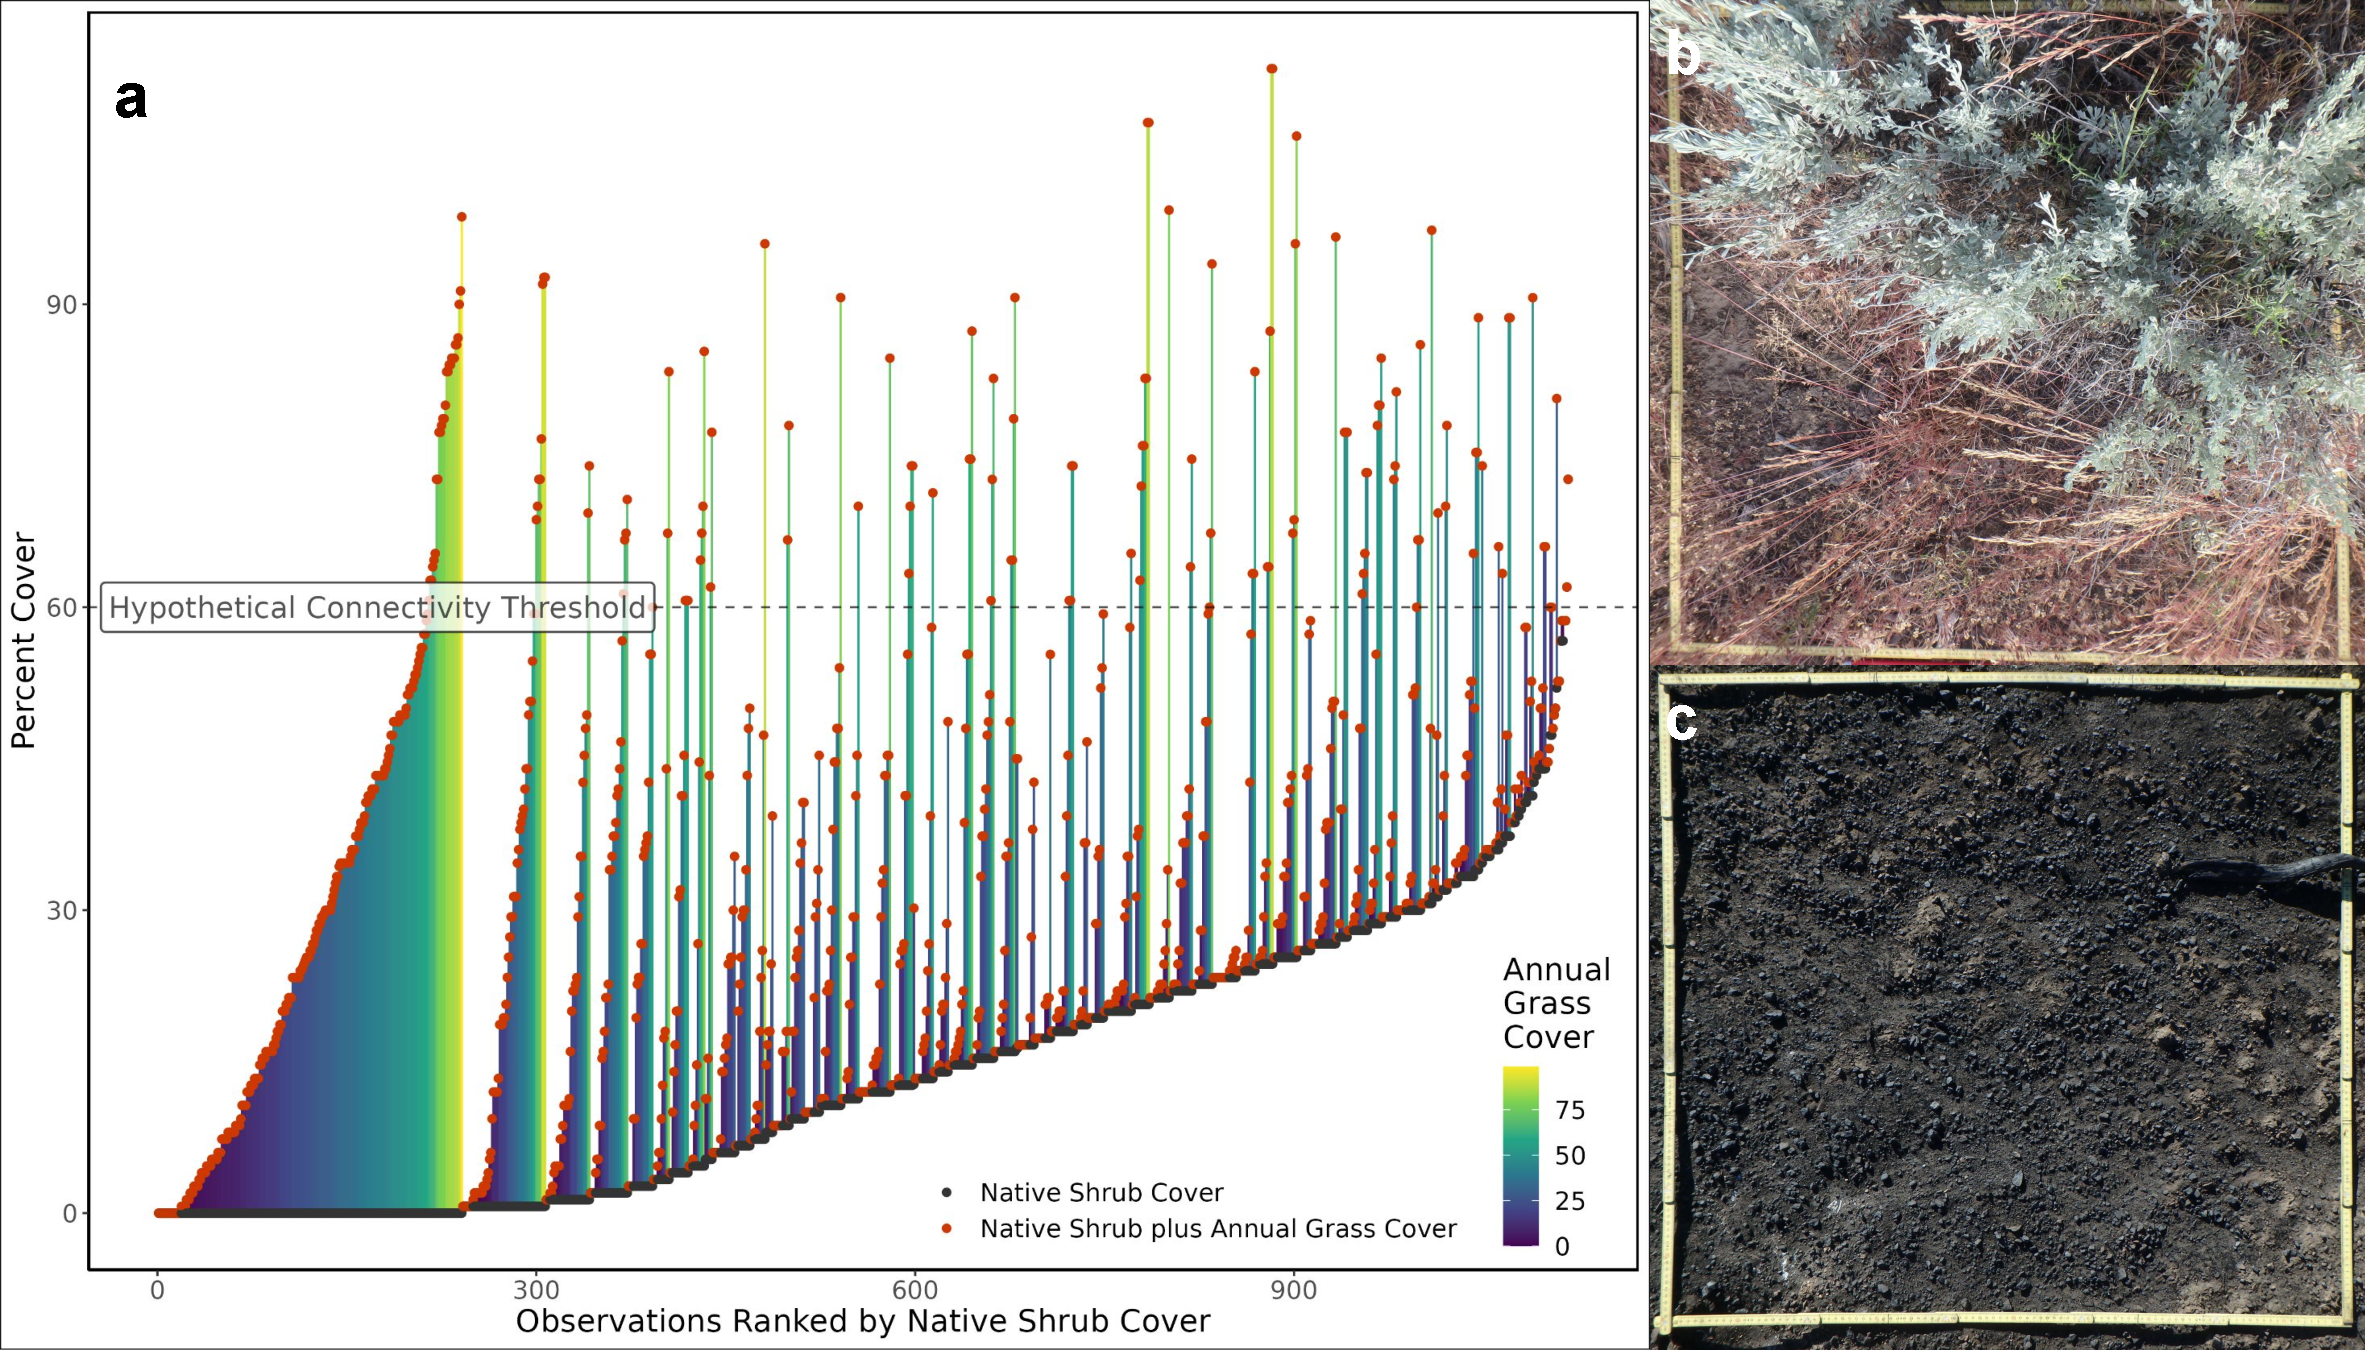
\includegraphics{images/fig2_seed_bank.pdf}
\caption{.}
\end{figure}

\newpage

\begin{figure}
\centering
\includegraphics{images/conceptual_figure.png}
\caption{.}
\end{figure}

\newpage

\begin{figure}
\centering
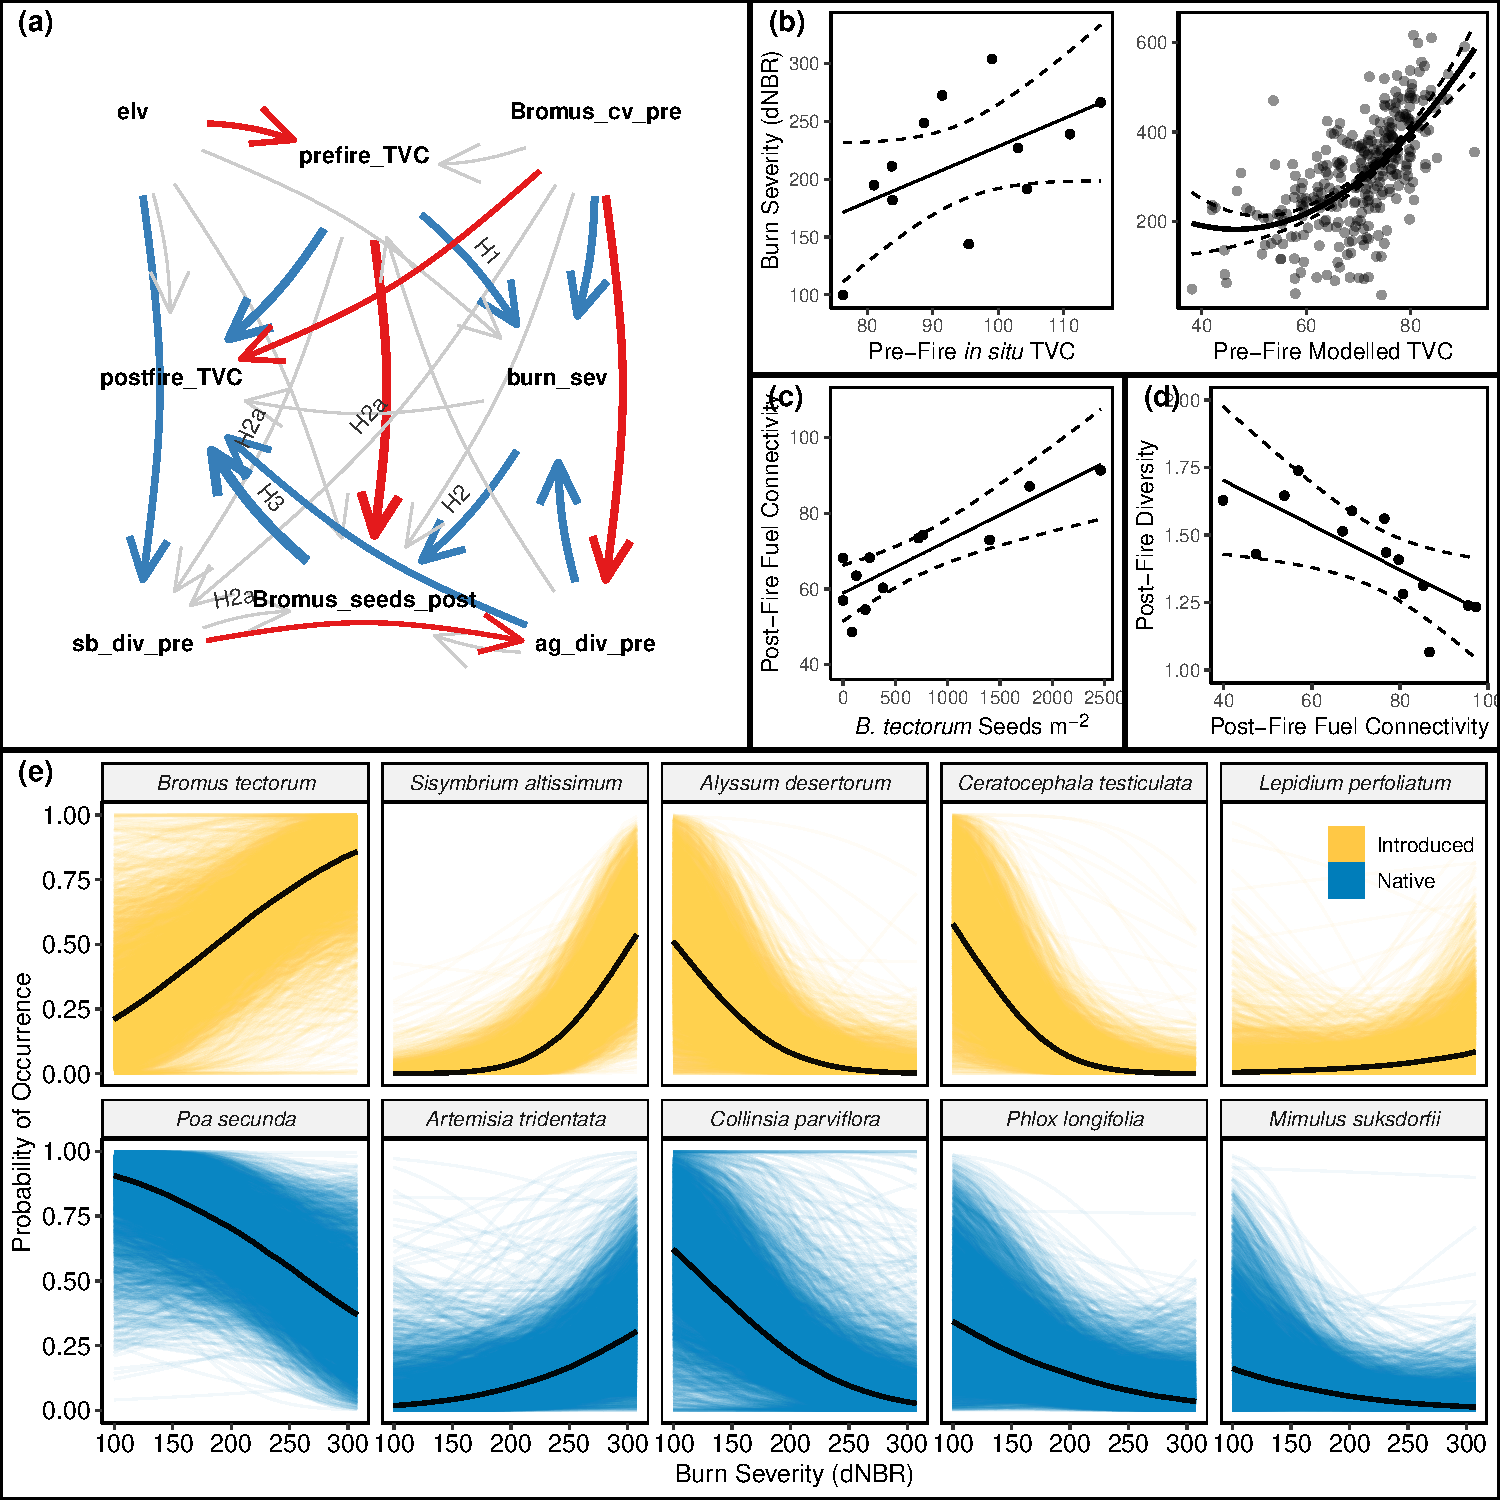
\includegraphics{images/big_plot_v2.pdf}
\caption{.}
\end{figure}

\end{document}
